% Options for packages loaded elsewhere
\PassOptionsToPackage{unicode}{hyperref}
\PassOptionsToPackage{hyphens}{url}
\PassOptionsToPackage{dvipsnames,svgnames,x11names}{xcolor}
%
\documentclass[
  letterpaper,
  DIV=11,
  numbers=noendperiod]{scrartcl}

\usepackage{amsmath,amssymb}
\usepackage{iftex}
\ifPDFTeX
  \usepackage[T1]{fontenc}
  \usepackage[utf8]{inputenc}
  \usepackage{textcomp} % provide euro and other symbols
\else % if luatex or xetex
  \usepackage{unicode-math}
  \defaultfontfeatures{Scale=MatchLowercase}
  \defaultfontfeatures[\rmfamily]{Ligatures=TeX,Scale=1}
\fi
\usepackage{lmodern}
\ifPDFTeX\else  
    % xetex/luatex font selection
\fi
% Use upquote if available, for straight quotes in verbatim environments
\IfFileExists{upquote.sty}{\usepackage{upquote}}{}
\IfFileExists{microtype.sty}{% use microtype if available
  \usepackage[]{microtype}
  \UseMicrotypeSet[protrusion]{basicmath} % disable protrusion for tt fonts
}{}
\makeatletter
\@ifundefined{KOMAClassName}{% if non-KOMA class
  \IfFileExists{parskip.sty}{%
    \usepackage{parskip}
  }{% else
    \setlength{\parindent}{0pt}
    \setlength{\parskip}{6pt plus 2pt minus 1pt}}
}{% if KOMA class
  \KOMAoptions{parskip=half}}
\makeatother
\usepackage{xcolor}
\setlength{\emergencystretch}{3em} % prevent overfull lines
\setcounter{secnumdepth}{5}
% Make \paragraph and \subparagraph free-standing
\makeatletter
\ifx\paragraph\undefined\else
  \let\oldparagraph\paragraph
  \renewcommand{\paragraph}{
    \@ifstar
      \xxxParagraphStar
      \xxxParagraphNoStar
  }
  \newcommand{\xxxParagraphStar}[1]{\oldparagraph*{#1}\mbox{}}
  \newcommand{\xxxParagraphNoStar}[1]{\oldparagraph{#1}\mbox{}}
\fi
\ifx\subparagraph\undefined\else
  \let\oldsubparagraph\subparagraph
  \renewcommand{\subparagraph}{
    \@ifstar
      \xxxSubParagraphStar
      \xxxSubParagraphNoStar
  }
  \newcommand{\xxxSubParagraphStar}[1]{\oldsubparagraph*{#1}\mbox{}}
  \newcommand{\xxxSubParagraphNoStar}[1]{\oldsubparagraph{#1}\mbox{}}
\fi
\makeatother

\usepackage{color}
\usepackage{fancyvrb}
\newcommand{\VerbBar}{|}
\newcommand{\VERB}{\Verb[commandchars=\\\{\}]}
\DefineVerbatimEnvironment{Highlighting}{Verbatim}{commandchars=\\\{\}}
% Add ',fontsize=\small' for more characters per line
\usepackage{framed}
\definecolor{shadecolor}{RGB}{241,243,245}
\newenvironment{Shaded}{\begin{snugshade}}{\end{snugshade}}
\newcommand{\AlertTok}[1]{\textcolor[rgb]{0.68,0.00,0.00}{#1}}
\newcommand{\AnnotationTok}[1]{\textcolor[rgb]{0.37,0.37,0.37}{#1}}
\newcommand{\AttributeTok}[1]{\textcolor[rgb]{0.40,0.45,0.13}{#1}}
\newcommand{\BaseNTok}[1]{\textcolor[rgb]{0.68,0.00,0.00}{#1}}
\newcommand{\BuiltInTok}[1]{\textcolor[rgb]{0.00,0.23,0.31}{#1}}
\newcommand{\CharTok}[1]{\textcolor[rgb]{0.13,0.47,0.30}{#1}}
\newcommand{\CommentTok}[1]{\textcolor[rgb]{0.37,0.37,0.37}{#1}}
\newcommand{\CommentVarTok}[1]{\textcolor[rgb]{0.37,0.37,0.37}{\textit{#1}}}
\newcommand{\ConstantTok}[1]{\textcolor[rgb]{0.56,0.35,0.01}{#1}}
\newcommand{\ControlFlowTok}[1]{\textcolor[rgb]{0.00,0.23,0.31}{\textbf{#1}}}
\newcommand{\DataTypeTok}[1]{\textcolor[rgb]{0.68,0.00,0.00}{#1}}
\newcommand{\DecValTok}[1]{\textcolor[rgb]{0.68,0.00,0.00}{#1}}
\newcommand{\DocumentationTok}[1]{\textcolor[rgb]{0.37,0.37,0.37}{\textit{#1}}}
\newcommand{\ErrorTok}[1]{\textcolor[rgb]{0.68,0.00,0.00}{#1}}
\newcommand{\ExtensionTok}[1]{\textcolor[rgb]{0.00,0.23,0.31}{#1}}
\newcommand{\FloatTok}[1]{\textcolor[rgb]{0.68,0.00,0.00}{#1}}
\newcommand{\FunctionTok}[1]{\textcolor[rgb]{0.28,0.35,0.67}{#1}}
\newcommand{\ImportTok}[1]{\textcolor[rgb]{0.00,0.46,0.62}{#1}}
\newcommand{\InformationTok}[1]{\textcolor[rgb]{0.37,0.37,0.37}{#1}}
\newcommand{\KeywordTok}[1]{\textcolor[rgb]{0.00,0.23,0.31}{\textbf{#1}}}
\newcommand{\NormalTok}[1]{\textcolor[rgb]{0.00,0.23,0.31}{#1}}
\newcommand{\OperatorTok}[1]{\textcolor[rgb]{0.37,0.37,0.37}{#1}}
\newcommand{\OtherTok}[1]{\textcolor[rgb]{0.00,0.23,0.31}{#1}}
\newcommand{\PreprocessorTok}[1]{\textcolor[rgb]{0.68,0.00,0.00}{#1}}
\newcommand{\RegionMarkerTok}[1]{\textcolor[rgb]{0.00,0.23,0.31}{#1}}
\newcommand{\SpecialCharTok}[1]{\textcolor[rgb]{0.37,0.37,0.37}{#1}}
\newcommand{\SpecialStringTok}[1]{\textcolor[rgb]{0.13,0.47,0.30}{#1}}
\newcommand{\StringTok}[1]{\textcolor[rgb]{0.13,0.47,0.30}{#1}}
\newcommand{\VariableTok}[1]{\textcolor[rgb]{0.07,0.07,0.07}{#1}}
\newcommand{\VerbatimStringTok}[1]{\textcolor[rgb]{0.13,0.47,0.30}{#1}}
\newcommand{\WarningTok}[1]{\textcolor[rgb]{0.37,0.37,0.37}{\textit{#1}}}

\providecommand{\tightlist}{%
  \setlength{\itemsep}{0pt}\setlength{\parskip}{0pt}}\usepackage{longtable,booktabs,array}
\usepackage{calc} % for calculating minipage widths
% Correct order of tables after \paragraph or \subparagraph
\usepackage{etoolbox}
\makeatletter
\patchcmd\longtable{\par}{\if@noskipsec\mbox{}\fi\par}{}{}
\makeatother
% Allow footnotes in longtable head/foot
\IfFileExists{footnotehyper.sty}{\usepackage{footnotehyper}}{\usepackage{footnote}}
\makesavenoteenv{longtable}
\usepackage{graphicx}
\makeatletter
\newsavebox\pandoc@box
\newcommand*\pandocbounded[1]{% scales image to fit in text height/width
  \sbox\pandoc@box{#1}%
  \Gscale@div\@tempa{\textheight}{\dimexpr\ht\pandoc@box+\dp\pandoc@box\relax}%
  \Gscale@div\@tempb{\linewidth}{\wd\pandoc@box}%
  \ifdim\@tempb\p@<\@tempa\p@\let\@tempa\@tempb\fi% select the smaller of both
  \ifdim\@tempa\p@<\p@\scalebox{\@tempa}{\usebox\pandoc@box}%
  \else\usebox{\pandoc@box}%
  \fi%
}
% Set default figure placement to htbp
\def\fps@figure{htbp}
\makeatother
% definitions for citeproc citations
\NewDocumentCommand\citeproctext{}{}
\NewDocumentCommand\citeproc{mm}{%
  \begingroup\def\citeproctext{#2}\cite{#1}\endgroup}
\makeatletter
 % allow citations to break across lines
 \let\@cite@ofmt\@firstofone
 % avoid brackets around text for \cite:
 \def\@biblabel#1{}
 \def\@cite#1#2{{#1\if@tempswa , #2\fi}}
\makeatother
\newlength{\cslhangindent}
\setlength{\cslhangindent}{1.5em}
\newlength{\csllabelwidth}
\setlength{\csllabelwidth}{3em}
\newenvironment{CSLReferences}[2] % #1 hanging-indent, #2 entry-spacing
 {\begin{list}{}{%
  \setlength{\itemindent}{0pt}
  \setlength{\leftmargin}{0pt}
  \setlength{\parsep}{0pt}
  % turn on hanging indent if param 1 is 1
  \ifodd #1
   \setlength{\leftmargin}{\cslhangindent}
   \setlength{\itemindent}{-1\cslhangindent}
  \fi
  % set entry spacing
  \setlength{\itemsep}{#2\baselineskip}}}
 {\end{list}}
\usepackage{calc}
\newcommand{\CSLBlock}[1]{\hfill\break\parbox[t]{\linewidth}{\strut\ignorespaces#1\strut}}
\newcommand{\CSLLeftMargin}[1]{\parbox[t]{\csllabelwidth}{\strut#1\strut}}
\newcommand{\CSLRightInline}[1]{\parbox[t]{\linewidth - \csllabelwidth}{\strut#1\strut}}
\newcommand{\CSLIndent}[1]{\hspace{\cslhangindent}#1}

\KOMAoption{captions}{tableheading}
\makeatletter
\@ifpackageloaded{caption}{}{\usepackage{caption}}
\AtBeginDocument{%
\ifdefined\contentsname
  \renewcommand*\contentsname{Table of contents}
\else
  \newcommand\contentsname{Table of contents}
\fi
\ifdefined\listfigurename
  \renewcommand*\listfigurename{List of Figures}
\else
  \newcommand\listfigurename{List of Figures}
\fi
\ifdefined\listtablename
  \renewcommand*\listtablename{List of Tables}
\else
  \newcommand\listtablename{List of Tables}
\fi
\ifdefined\figurename
  \renewcommand*\figurename{Figure}
\else
  \newcommand\figurename{Figure}
\fi
\ifdefined\tablename
  \renewcommand*\tablename{Table}
\else
  \newcommand\tablename{Table}
\fi
}
\@ifpackageloaded{float}{}{\usepackage{float}}
\floatstyle{ruled}
\@ifundefined{c@chapter}{\newfloat{codelisting}{h}{lop}}{\newfloat{codelisting}{h}{lop}[chapter]}
\floatname{codelisting}{Listing}
\newcommand*\listoflistings{\listof{codelisting}{List of Listings}}
\makeatother
\makeatletter
\makeatother
\makeatletter
\@ifpackageloaded{caption}{}{\usepackage{caption}}
\@ifpackageloaded{subcaption}{}{\usepackage{subcaption}}
\makeatother

\usepackage{bookmark}

\IfFileExists{xurl.sty}{\usepackage{xurl}}{} % add URL line breaks if available
\urlstyle{same} % disable monospaced font for URLs
\hypersetup{
  pdftitle={Population},
  pdfauthor={Jin Myung Kim},
  colorlinks=true,
  linkcolor={blue},
  filecolor={Maroon},
  citecolor={Blue},
  urlcolor={Blue},
  pdfcreator={LaTeX via pandoc}}


\title{Population}
\author{Jin Myung Kim}
\date{2025-07-19}

\begin{document}
\maketitle

\renewcommand*\contentsname{Table of contents}
{
\hypersetup{linkcolor=}
\setcounter{tocdepth}{2}
\tableofcontents
}

\section{Introduction}\label{introduction}

In an effort to reduce both domestic consumption and regional opium
production, the Chinese government launched the Opium Replacement
Program (ORP) in 2006. This initiative was designed to provide funding
for Chinese companies to invest in opium-cultivating regions of Laos and
Myanmar by supporting the transition of local farmers to cash crops such
as rubber, maize, and sugarcane, thereby fostering broader
socio-economic development in affected areas (J. Lu and Dwyer 2023;
UNODC 2015; TNI 2010). Initially proposed as part of China's broader
``Going Out'' strategy in the early 2000s to encourage overseas
investment, the ORP was officially initiated in 2004 and subsequently
formalized and expanded in 2006 when it was incorporated into China's
five-year plan with dedicated funding and policy support. Its stated aim
is to replace opium cultivation in the Golden Triangle with licit,
high-value cash crops, thus improving local livelihoods and promoting
economic cooperation. To incentivize participation, Chinese companies
involved in the program are offered tax exemptions within import quotas,
along with subsidies and interest-free loans (TNI 2010; Cohen 2009; J.
N. Lu 2019). Approximately 7.2 million USD (50 million RMB) in central
funding, supplemented by 4.3 million USD (30 million RMB) from
provincial matching funds, was allocated to the program. Companies must
manage large-scale investment projects covering over 600 hectares
(10,000 mu) to qualify, and these funds support the establishment of
plantations for crops such as rubber, maize, and sugarcane.

Despite the policy's initial aim of nudging firms to invest directly to
the opium farmers, firms had lots of autonomy throughout the investment
activity. To be more specific, firms established locations where it
favors firms' business operations rather than cooperate directly with
opium farmers. By conducting several interviews with different
stakeholders, J. N. Lu (2019) argues that the ORP attempts `'replacement
by displacement'\,'. That is, the replacement of opium cultivation is
achieved by drawing opium farmers out of opium fields by providing labor
opportunities in alternative crop plantations which are often
established at regions near road and with low elevation.

\subsection{Experimental Design}\label{experimental-design}

\textbf{Main Hypothesis:} The introduction of the ORP program decreased
the opium cultivation.

\textbf{Ideal experimental design:} Randomly pick villages (that
cultivate opium) and introduce ORP in some villages and leave rest of
the villages untouched.

\textbf{Issue:}

\begin{itemize}
\tightlist
\item
  Randomization: The treatment are not received randomly. Villages are
  treated based on whether the village is suitable for business
  operations (i.e.~low elevation, near road, etc.). Thus, we might want
  to characterize locations suitable for ORP alternative crop
  plantation, using distance to road, slope, and elevation.
\end{itemize}

\textbf{Refined Hypothesis:} Controlling for geographic accessibility
and baseline opium risk, village exposed to ORP experienced a greater
reduction in opium cultivation compared to similar, non-treated
villages.

\textbf{Mechanism:}

\begin{itemize}
\item
  First-order Impact

  \begin{enumerate}
  \def\labelenumi{\arabic{enumi}.}
  \tightlist
  \item
    Local laborers shift from opium cultivation to wage labor on these
    plantations.
  \item
    Farmers/opium farmers migrate to ORP zones for better opportunities
    (replacement by displacement).
  \end{enumerate}
\item
  Second-order Impact

  \begin{enumerate}
  \def\labelenumi{\arabic{enumi}.}
  \tightlist
  \item
    Schooling and child labor: with stable ORP income, some households
    pull children from labor to school (Sviatschi 2022; UNODC 2005)
  \end{enumerate}
\end{itemize}

ORP likely impacted population dynamics in Laos, especially through the
relocation of labor from upland opium-growing areas to lowland
agricultural and economic centers. We will explore such dynamics in the
following section to better characterize such characteristics and check
the possibility of the `'replacement by displacement'\,' mechanism.

\textbf{Population and Housing Census.} To understand these changes, we
first analyze Laos' Population and Housing Census (2005) to establish a
pre-ORP baseline. We assess how population, population density, and
poverty levels relate to terrain characteristics (elevation, slope),
road accessibility, and how they evolved between 2005 and 2015.

\textbf{World Pop.} Then we will use WorldPop data, which is trained
using machine learning technique to simulate the population distribution
between 2000 and 2020. This will add additional information on the
population dynamics to the Population Housing Census information which
is limited to only 2005 and 2015.

\textbf{ORP Program.} Then we will check whether the observed population
dynamic is affected by ORP programs using official ORP records.

\section{Population and Housing
Census}\label{population-and-housing-census}

\subsection{Baseline Patterns in 2005 and
2015}\label{baseline-patterns-in-2005-and-2015}

\begin{itemize}
\item
  \textbf{Population and density were higher in accessible,
  low-elevation/slope areas}

  \begin{itemize}
  \item
    Villages located at lower elevations, with gentler slopes, and
    closer to national or provincial roads had significantly higher
    population and population density. Among these characteristics,
    slope showed the strongest negative association, followed by
    elevation and road distance.
  \item
    \emph{Slope, elevation, and distance to road should be treated as
    core baseline covariates.}
  \end{itemize}
\end{itemize}

\begin{Shaded}
\begin{Highlighting}[]
\CommentTok{\# Fit linear model}
\NormalTok{model\_slope }\OtherTok{\textless{}{-}} \FunctionTok{lm}\NormalTok{(}\FunctionTok{log}\NormalTok{(population) }\SpecialCharTok{\textasciitilde{}}\NormalTok{ mean\_slope, }\AttributeTok{data =}\NormalTok{ v\_2005)}
\NormalTok{summary\_slope }\OtherTok{\textless{}{-}} \FunctionTok{summary}\NormalTok{(model\_slope)}

\CommentTok{\# Extract values}
\NormalTok{coef\_slope }\OtherTok{\textless{}{-}}\NormalTok{ summary\_slope}\SpecialCharTok{$}\NormalTok{coefficients[}\StringTok{"mean\_slope"}\NormalTok{, }\StringTok{"Estimate"}\NormalTok{]}
\NormalTok{se\_slope   }\OtherTok{\textless{}{-}}\NormalTok{ summary\_slope}\SpecialCharTok{$}\NormalTok{coefficients[}\StringTok{"mean\_slope"}\NormalTok{, }\StringTok{"Std. Error"}\NormalTok{]}
\NormalTok{r2\_slope   }\OtherTok{\textless{}{-}}\NormalTok{ summary\_slope}\SpecialCharTok{$}\NormalTok{r.squared}

\CommentTok{\# Format label}
\NormalTok{label\_slope }\OtherTok{\textless{}{-}} \FunctionTok{sprintf}\NormalTok{(}\StringTok{"β = \%.3f (SE = \%.3f)}\SpecialCharTok{\textbackslash{}n}\StringTok{R² = \%.3f"}\NormalTok{, coef\_slope, se\_slope, r2\_slope)}

\CommentTok{\# Plot}
\NormalTok{p1 }\OtherTok{\textless{}{-}} \FunctionTok{ggplot}\NormalTok{(v\_2005, }\FunctionTok{aes}\NormalTok{(}\AttributeTok{x =}\NormalTok{ mean\_slope, }\AttributeTok{y =} \FunctionTok{log}\NormalTok{(population))) }\SpecialCharTok{+}
  \FunctionTok{geom\_point}\NormalTok{(}\AttributeTok{alpha =} \FloatTok{0.5}\NormalTok{) }\SpecialCharTok{+}
  \FunctionTok{geom\_smooth}\NormalTok{(}\AttributeTok{method =} \StringTok{"lm"}\NormalTok{, }\AttributeTok{color =} \StringTok{"blue"}\NormalTok{, }\AttributeTok{se =} \ConstantTok{TRUE}\NormalTok{) }\SpecialCharTok{+}
  \FunctionTok{annotate}\NormalTok{(}\StringTok{"text"}\NormalTok{, }\AttributeTok{x =} \ConstantTok{Inf}\NormalTok{, }\AttributeTok{y =} \ConstantTok{Inf}\NormalTok{, }\AttributeTok{label =}\NormalTok{ label\_slope, }\AttributeTok{hjust =} \FloatTok{1.1}\NormalTok{, }\AttributeTok{vjust =} \FloatTok{1.5}\NormalTok{, }\AttributeTok{size =} \DecValTok{5}\NormalTok{) }\SpecialCharTok{+}
  \FunctionTok{labs}\NormalTok{(}
    \AttributeTok{title =} \StringTok{"Slope and Population"}\NormalTok{,}
    \AttributeTok{x =} \StringTok{"Mean Slope (°)"}\NormalTok{,}
    \AttributeTok{y =} \StringTok{"Log Population"}
\NormalTok{  ) }\SpecialCharTok{+}
  \FunctionTok{theme\_bw}\NormalTok{()}

\CommentTok{\# Fit linear model}
\NormalTok{model\_elev }\OtherTok{\textless{}{-}} \FunctionTok{lm}\NormalTok{(}\FunctionTok{log}\NormalTok{(population) }\SpecialCharTok{\textasciitilde{}}\NormalTok{ mean\_elev, }\AttributeTok{data =}\NormalTok{ v\_2005)}
\NormalTok{summary\_elev }\OtherTok{\textless{}{-}} \FunctionTok{summary}\NormalTok{(model\_elev)}

\CommentTok{\# Extract values}
\NormalTok{coef\_elev }\OtherTok{\textless{}{-}}\NormalTok{ summary\_elev}\SpecialCharTok{$}\NormalTok{coefficients[}\StringTok{"mean\_elev"}\NormalTok{, }\StringTok{"Estimate"}\NormalTok{]}
\NormalTok{se\_elev   }\OtherTok{\textless{}{-}}\NormalTok{ summary\_elev}\SpecialCharTok{$}\NormalTok{coefficients[}\StringTok{"mean\_elev"}\NormalTok{, }\StringTok{"Std. Error"}\NormalTok{]}
\NormalTok{r2\_elev   }\OtherTok{\textless{}{-}}\NormalTok{ summary\_elev}\SpecialCharTok{$}\NormalTok{r.squared}

\CommentTok{\# Format label}
\NormalTok{label\_elev }\OtherTok{\textless{}{-}} \FunctionTok{sprintf}\NormalTok{(}\StringTok{"β = \%.3f (SE = \%.3f)}\SpecialCharTok{\textbackslash{}n}\StringTok{R² = \%.3f"}\NormalTok{, coef\_elev, se\_elev, r2\_elev)}

\CommentTok{\# Plot}
\NormalTok{p2 }\OtherTok{\textless{}{-}} \FunctionTok{ggplot}\NormalTok{(v\_2005, }\FunctionTok{aes}\NormalTok{(}\AttributeTok{x =}\NormalTok{ mean\_elev, }\AttributeTok{y =} \FunctionTok{log}\NormalTok{(population))) }\SpecialCharTok{+}
  \FunctionTok{geom\_point}\NormalTok{(}\AttributeTok{alpha =} \FloatTok{0.5}\NormalTok{) }\SpecialCharTok{+}
  \FunctionTok{geom\_smooth}\NormalTok{(}\AttributeTok{method =} \StringTok{"lm"}\NormalTok{, }\AttributeTok{color =} \StringTok{"blue"}\NormalTok{, }\AttributeTok{se =} \ConstantTok{TRUE}\NormalTok{) }\SpecialCharTok{+}
  \FunctionTok{annotate}\NormalTok{(}\StringTok{"text"}\NormalTok{, }\AttributeTok{x =} \ConstantTok{Inf}\NormalTok{, }\AttributeTok{y =} \ConstantTok{Inf}\NormalTok{, }\AttributeTok{label =}\NormalTok{ label\_elev, }\AttributeTok{hjust =} \FloatTok{1.1}\NormalTok{, }\AttributeTok{vjust =} \FloatTok{1.5}\NormalTok{, }\AttributeTok{size =} \DecValTok{5}\NormalTok{) }\SpecialCharTok{+}
  \FunctionTok{labs}\NormalTok{(}
    \AttributeTok{title =} \StringTok{"Elevation and opulation"}\NormalTok{,}
    \AttributeTok{x =} \StringTok{"Mean Elevation (m)"}\NormalTok{,}
    \AttributeTok{y =} \StringTok{"Log Population"}
\NormalTok{  ) }\SpecialCharTok{+} 
  \FunctionTok{theme\_bw}\NormalTok{()}

\CommentTok{\# Fit linear model with log{-}transformed mean\_dist}
\NormalTok{model\_log\_dist }\OtherTok{\textless{}{-}} \FunctionTok{lm}\NormalTok{(}\FunctionTok{log}\NormalTok{(population) }\SpecialCharTok{\textasciitilde{}} \FunctionTok{log}\NormalTok{(mean\_dist), }\AttributeTok{data =}\NormalTok{ v\_2005)}
\NormalTok{summary\_log\_dist }\OtherTok{\textless{}{-}} \FunctionTok{summary}\NormalTok{(model\_log\_dist)}

\CommentTok{\# Extract values}
\NormalTok{coef\_log\_dist }\OtherTok{\textless{}{-}}\NormalTok{ summary\_log\_dist}\SpecialCharTok{$}\NormalTok{coefficients[}\StringTok{"log(mean\_dist)"}\NormalTok{, }\StringTok{"Estimate"}\NormalTok{]}
\NormalTok{se\_log\_dist   }\OtherTok{\textless{}{-}}\NormalTok{ summary\_log\_dist}\SpecialCharTok{$}\NormalTok{coefficients[}\StringTok{"log(mean\_dist)"}\NormalTok{, }\StringTok{"Std. Error"}\NormalTok{]}
\NormalTok{r2\_log\_dist   }\OtherTok{\textless{}{-}}\NormalTok{ summary\_log\_dist}\SpecialCharTok{$}\NormalTok{r.squared}

\CommentTok{\# Format annotation label}
\NormalTok{label\_log\_dist }\OtherTok{\textless{}{-}} \FunctionTok{sprintf}\NormalTok{(}\StringTok{"β = \%.3f (SE = \%.3f)}\SpecialCharTok{\textbackslash{}n}\StringTok{R² = \%.3f"}\NormalTok{, coef\_log\_dist, se\_log\_dist, r2\_log\_dist)}

\CommentTok{\# Plot}
\NormalTok{p3 }\OtherTok{\textless{}{-}} \FunctionTok{ggplot}\NormalTok{(}\AttributeTok{data =}\NormalTok{ v\_2005, }\FunctionTok{aes}\NormalTok{(}\AttributeTok{x =} \FunctionTok{log}\NormalTok{(mean\_dist), }\AttributeTok{y =} \FunctionTok{log}\NormalTok{(population))) }\SpecialCharTok{+}
  \FunctionTok{geom\_point}\NormalTok{(}\AttributeTok{alpha =} \FloatTok{0.5}\NormalTok{) }\SpecialCharTok{+}
  \FunctionTok{geom\_smooth}\NormalTok{(}\AttributeTok{method =} \StringTok{"lm"}\NormalTok{, }\AttributeTok{color =} \StringTok{"blue"}\NormalTok{, }\AttributeTok{se =} \ConstantTok{TRUE}\NormalTok{) }\SpecialCharTok{+}
  \FunctionTok{annotate}\NormalTok{(}\StringTok{"text"}\NormalTok{, }\AttributeTok{x =} \ConstantTok{Inf}\NormalTok{, }\AttributeTok{y =} \ConstantTok{Inf}\NormalTok{, }\AttributeTok{label =}\NormalTok{ label\_log\_dist, }\AttributeTok{hjust =} \FloatTok{1.1}\NormalTok{, }\AttributeTok{vjust =} \FloatTok{1.5}\NormalTok{, }\AttributeTok{size =} \DecValTok{5}\NormalTok{) }\SpecialCharTok{+}
  \FunctionTok{labs}\NormalTok{(}
    \AttributeTok{title =} \StringTok{"Distance to Road and Population"}\NormalTok{,}
    \AttributeTok{x =} \StringTok{"Log Mean Distance to Road (m)"}\NormalTok{,}
    \AttributeTok{y =} \StringTok{"Log Population"}
\NormalTok{  ) }\SpecialCharTok{+} 
  \FunctionTok{theme\_bw}\NormalTok{()}

\CommentTok{\# Fit linear model}
\NormalTok{model\_slope }\OtherTok{\textless{}{-}} \FunctionTok{lm}\NormalTok{(}\FunctionTok{log}\NormalTok{(population\_density) }\SpecialCharTok{\textasciitilde{}}\NormalTok{ mean\_slope, }\AttributeTok{data =}\NormalTok{ v\_2005)}
\NormalTok{summary\_slope }\OtherTok{\textless{}{-}} \FunctionTok{summary}\NormalTok{(model\_slope)}

\CommentTok{\# Extract values}
\NormalTok{coef\_slope }\OtherTok{\textless{}{-}}\NormalTok{ summary\_slope}\SpecialCharTok{$}\NormalTok{coefficients[}\StringTok{"mean\_slope"}\NormalTok{, }\StringTok{"Estimate"}\NormalTok{]}
\NormalTok{se\_slope   }\OtherTok{\textless{}{-}}\NormalTok{ summary\_slope}\SpecialCharTok{$}\NormalTok{coefficients[}\StringTok{"mean\_slope"}\NormalTok{, }\StringTok{"Std. Error"}\NormalTok{]}
\NormalTok{r2\_slope   }\OtherTok{\textless{}{-}}\NormalTok{ summary\_slope}\SpecialCharTok{$}\NormalTok{r.squared}

\CommentTok{\# Format label}
\NormalTok{label\_slope }\OtherTok{\textless{}{-}} \FunctionTok{sprintf}\NormalTok{(}\StringTok{"β = \%.3f (SE = \%.3f)}\SpecialCharTok{\textbackslash{}n}\StringTok{R² = \%.3f"}\NormalTok{, coef\_slope, se\_slope, r2\_slope)}

\CommentTok{\# Plot}
\NormalTok{p4 }\OtherTok{\textless{}{-}} \FunctionTok{ggplot}\NormalTok{(v\_2005, }\FunctionTok{aes}\NormalTok{(}\AttributeTok{x =}\NormalTok{ mean\_slope, }\AttributeTok{y =} \FunctionTok{log}\NormalTok{(population\_density))) }\SpecialCharTok{+}
  \FunctionTok{geom\_point}\NormalTok{(}\AttributeTok{alpha =} \FloatTok{0.5}\NormalTok{) }\SpecialCharTok{+}
  \FunctionTok{geom\_smooth}\NormalTok{(}\AttributeTok{method =} \StringTok{"lm"}\NormalTok{, }\AttributeTok{color =} \StringTok{"blue"}\NormalTok{, }\AttributeTok{se =} \ConstantTok{TRUE}\NormalTok{) }\SpecialCharTok{+}
  \FunctionTok{annotate}\NormalTok{(}\StringTok{"text"}\NormalTok{, }\AttributeTok{x =} \ConstantTok{Inf}\NormalTok{, }\AttributeTok{y =} \ConstantTok{Inf}\NormalTok{, }\AttributeTok{label =}\NormalTok{ label\_slope, }\AttributeTok{hjust =} \FloatTok{1.1}\NormalTok{, }\AttributeTok{vjust =} \FloatTok{1.5}\NormalTok{, }\AttributeTok{size =} \DecValTok{5}\NormalTok{) }\SpecialCharTok{+}
  \FunctionTok{labs}\NormalTok{(}
    \AttributeTok{title =} \StringTok{"Slope and Population Density"}\NormalTok{,}
    \AttributeTok{x =} \StringTok{"Mean Slope (°)"}\NormalTok{,}
    \AttributeTok{y =} \StringTok{"Log Population Density"}
\NormalTok{  ) }\SpecialCharTok{+}
  \FunctionTok{theme\_bw}\NormalTok{()}

\CommentTok{\# Fit linear model}
\NormalTok{model\_elev }\OtherTok{\textless{}{-}} \FunctionTok{lm}\NormalTok{(}\FunctionTok{log}\NormalTok{(population\_density) }\SpecialCharTok{\textasciitilde{}}\NormalTok{ mean\_elev, }\AttributeTok{data =}\NormalTok{ v\_2005)}
\NormalTok{summary\_elev }\OtherTok{\textless{}{-}} \FunctionTok{summary}\NormalTok{(model\_elev)}

\CommentTok{\# Extract values}
\NormalTok{coef\_elev }\OtherTok{\textless{}{-}}\NormalTok{ summary\_elev}\SpecialCharTok{$}\NormalTok{coefficients[}\StringTok{"mean\_elev"}\NormalTok{, }\StringTok{"Estimate"}\NormalTok{]}
\NormalTok{se\_elev   }\OtherTok{\textless{}{-}}\NormalTok{ summary\_elev}\SpecialCharTok{$}\NormalTok{coefficients[}\StringTok{"mean\_elev"}\NormalTok{, }\StringTok{"Std. Error"}\NormalTok{]}
\NormalTok{r2\_elev   }\OtherTok{\textless{}{-}}\NormalTok{ summary\_elev}\SpecialCharTok{$}\NormalTok{r.squared}

\CommentTok{\# Format label}
\NormalTok{label\_elev }\OtherTok{\textless{}{-}} \FunctionTok{sprintf}\NormalTok{(}\StringTok{"β = \%.3f (SE = \%.3f)}\SpecialCharTok{\textbackslash{}n}\StringTok{R² = \%.3f"}\NormalTok{, coef\_elev, se\_elev, r2\_elev)}

\CommentTok{\# Plot}
\NormalTok{p5 }\OtherTok{\textless{}{-}} \FunctionTok{ggplot}\NormalTok{(v\_2005, }\FunctionTok{aes}\NormalTok{(}\AttributeTok{x =}\NormalTok{ mean\_elev, }\AttributeTok{y =} \FunctionTok{log}\NormalTok{(population\_density))) }\SpecialCharTok{+}
  \FunctionTok{geom\_point}\NormalTok{(}\AttributeTok{alpha =} \FloatTok{0.5}\NormalTok{) }\SpecialCharTok{+}
  \FunctionTok{geom\_smooth}\NormalTok{(}\AttributeTok{method =} \StringTok{"lm"}\NormalTok{, }\AttributeTok{color =} \StringTok{"blue"}\NormalTok{, }\AttributeTok{se =} \ConstantTok{TRUE}\NormalTok{) }\SpecialCharTok{+}
  \FunctionTok{annotate}\NormalTok{(}\StringTok{"text"}\NormalTok{, }\AttributeTok{x =} \ConstantTok{Inf}\NormalTok{, }\AttributeTok{y =} \ConstantTok{Inf}\NormalTok{, }\AttributeTok{label =}\NormalTok{ label\_elev, }\AttributeTok{hjust =} \FloatTok{1.1}\NormalTok{, }\AttributeTok{vjust =} \FloatTok{1.5}\NormalTok{, }\AttributeTok{size =} \DecValTok{5}\NormalTok{) }\SpecialCharTok{+}
  \FunctionTok{labs}\NormalTok{(}
    \AttributeTok{title =} \StringTok{"Elevation and Population Density"}\NormalTok{,}
    \AttributeTok{x =} \StringTok{"Mean Elevation (m)"}\NormalTok{,}
    \AttributeTok{y =} \StringTok{"Log Population Density"}
\NormalTok{  ) }\SpecialCharTok{+} 
  \FunctionTok{theme\_bw}\NormalTok{()}

\CommentTok{\# Fit linear model with log{-}transformed mean\_dist}
\NormalTok{model\_log\_dist }\OtherTok{\textless{}{-}} \FunctionTok{lm}\NormalTok{(}\FunctionTok{log}\NormalTok{(population\_density) }\SpecialCharTok{\textasciitilde{}} \FunctionTok{log}\NormalTok{(mean\_dist), }\AttributeTok{data =}\NormalTok{ v\_2005)}
\NormalTok{summary\_log\_dist }\OtherTok{\textless{}{-}} \FunctionTok{summary}\NormalTok{(model\_log\_dist)}

\CommentTok{\# Extract values}
\NormalTok{coef\_log\_dist }\OtherTok{\textless{}{-}}\NormalTok{ summary\_log\_dist}\SpecialCharTok{$}\NormalTok{coefficients[}\StringTok{"log(mean\_dist)"}\NormalTok{, }\StringTok{"Estimate"}\NormalTok{]}
\NormalTok{se\_log\_dist   }\OtherTok{\textless{}{-}}\NormalTok{ summary\_log\_dist}\SpecialCharTok{$}\NormalTok{coefficients[}\StringTok{"log(mean\_dist)"}\NormalTok{, }\StringTok{"Std. Error"}\NormalTok{]}
\NormalTok{r2\_log\_dist   }\OtherTok{\textless{}{-}}\NormalTok{ summary\_log\_dist}\SpecialCharTok{$}\NormalTok{r.squared}

\CommentTok{\# Format annotation label}
\NormalTok{label\_log\_dist }\OtherTok{\textless{}{-}} \FunctionTok{sprintf}\NormalTok{(}\StringTok{"β = \%.3f (SE = \%.3f)}\SpecialCharTok{\textbackslash{}n}\StringTok{R² = \%.3f"}\NormalTok{, coef\_log\_dist, se\_log\_dist, r2\_log\_dist)}

\CommentTok{\# Plot}
\NormalTok{p6 }\OtherTok{\textless{}{-}} \FunctionTok{ggplot}\NormalTok{(}\AttributeTok{data =}\NormalTok{ v\_2005, }\FunctionTok{aes}\NormalTok{(}\AttributeTok{x =} \FunctionTok{log}\NormalTok{(mean\_dist), }\AttributeTok{y =} \FunctionTok{log}\NormalTok{(population\_density))) }\SpecialCharTok{+}
  \FunctionTok{geom\_point}\NormalTok{(}\AttributeTok{alpha =} \FloatTok{0.5}\NormalTok{) }\SpecialCharTok{+}
  \FunctionTok{geom\_smooth}\NormalTok{(}\AttributeTok{method =} \StringTok{"lm"}\NormalTok{, }\AttributeTok{color =} \StringTok{"blue"}\NormalTok{, }\AttributeTok{se =} \ConstantTok{TRUE}\NormalTok{) }\SpecialCharTok{+}
  \FunctionTok{annotate}\NormalTok{(}\StringTok{"text"}\NormalTok{, }\AttributeTok{x =} \ConstantTok{Inf}\NormalTok{, }\AttributeTok{y =} \ConstantTok{Inf}\NormalTok{, }\AttributeTok{label =}\NormalTok{ label\_log\_dist, }\AttributeTok{hjust =} \FloatTok{1.1}\NormalTok{, }\AttributeTok{vjust =} \FloatTok{1.5}\NormalTok{, }\AttributeTok{size =} \DecValTok{5}\NormalTok{) }\SpecialCharTok{+}
  \FunctionTok{labs}\NormalTok{(}
    \AttributeTok{title =} \StringTok{"Distance to Road and Population Density"}\NormalTok{,}
    \AttributeTok{x =} \StringTok{"Log Mean Distance to Road (m)"}\NormalTok{,}
    \AttributeTok{y =} \StringTok{"Log Population Density"}
\NormalTok{  ) }\SpecialCharTok{+} 
  \FunctionTok{theme\_bw}\NormalTok{()}

\NormalTok{(p1 }\SpecialCharTok{+}\NormalTok{ p2 }\SpecialCharTok{+}\NormalTok{ p3) }\SpecialCharTok{/}\NormalTok{ (p4 }\SpecialCharTok{+}\NormalTok{ p5 }\SpecialCharTok{+}\NormalTok{ p6)}
\end{Highlighting}
\end{Shaded}

\pandocbounded{\includegraphics[keepaspectratio]{population_files/figure-pdf/unnamed-chunk-3-1.pdf}}

\pandocbounded{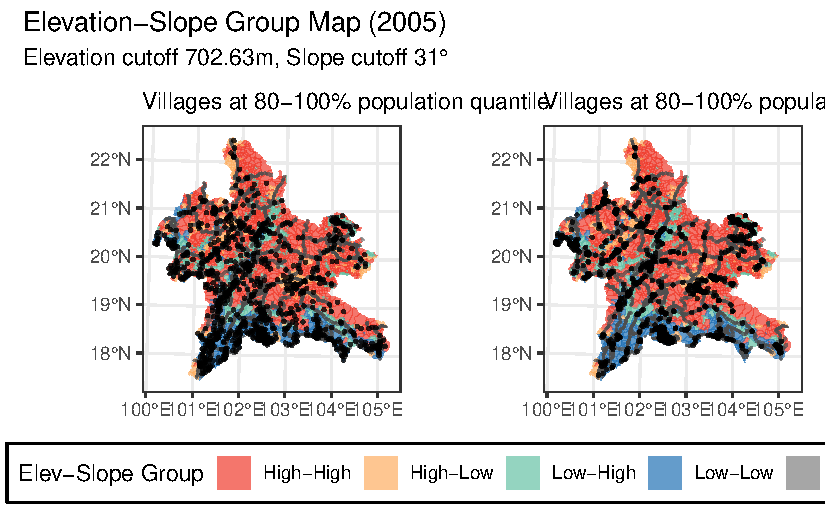
\includegraphics[keepaspectratio]{population_files/figure-pdf/unnamed-chunk-4-1.pdf}}

\pandocbounded{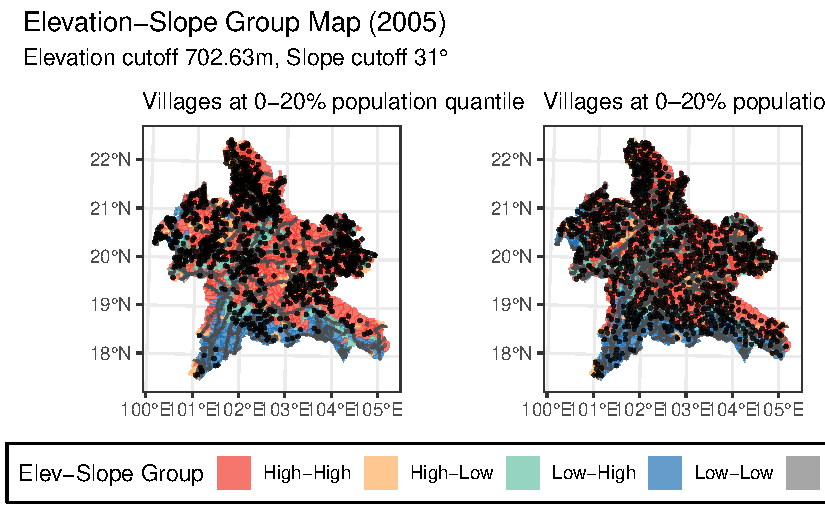
\includegraphics[keepaspectratio]{population_files/figure-pdf/unnamed-chunk-8-1.pdf}}

In order to simultaneously consider the relationship between population
and population density with elevation and slope, we categorized the
villages in Northern Laos by following classification:

\begin{itemize}
\item
  Slope: `'High Slope Village'\,' if the average slope of the village is
  greater than 31 (median average slope) and ``Low Slope Village''
  otherwise.
\item
  Elevation: `'High Elevation Village'\,' if the average mean of the
  village is greater than 702.63 meter and `'Low Elevation Village'\,'
  otherwise.
\end{itemize}

According to Administration et al. (1992) and UNODC (2001) opium poppy
cultivation are known to thrive in elevation above 700 meters and slope
between 20 to 40 degree. This coincides with the above classification.

Note: Figures above did not considered distance to road since there is a
strong correlation between distance to road and slope/elevation.

\begin{Shaded}
\begin{Highlighting}[]
\CommentTok{\# Fit linear model}
\NormalTok{model\_slope }\OtherTok{\textless{}{-}} \FunctionTok{lm}\NormalTok{(}\FunctionTok{log}\NormalTok{(mean\_dist) }\SpecialCharTok{\textasciitilde{}}\NormalTok{ mean\_slope, }\AttributeTok{data =}\NormalTok{ v\_2005)}
\NormalTok{summary\_slope }\OtherTok{\textless{}{-}} \FunctionTok{summary}\NormalTok{(model\_slope)}

\CommentTok{\# Extract values}
\NormalTok{coef\_slope }\OtherTok{\textless{}{-}}\NormalTok{ summary\_slope}\SpecialCharTok{$}\NormalTok{coefficients[}\StringTok{"mean\_slope"}\NormalTok{, }\StringTok{"Estimate"}\NormalTok{]}
\NormalTok{se\_slope   }\OtherTok{\textless{}{-}}\NormalTok{ summary\_slope}\SpecialCharTok{$}\NormalTok{coefficients[}\StringTok{"mean\_slope"}\NormalTok{, }\StringTok{"Std. Error"}\NormalTok{]}
\NormalTok{r2\_slope   }\OtherTok{\textless{}{-}}\NormalTok{ summary\_slope}\SpecialCharTok{$}\NormalTok{r.squared}

\CommentTok{\# Format label}
\NormalTok{label\_slope }\OtherTok{\textless{}{-}} \FunctionTok{sprintf}\NormalTok{(}\StringTok{"β = \%.3f (SE = \%.3f)}\SpecialCharTok{\textbackslash{}n}\StringTok{R² = \%.3f"}\NormalTok{, coef\_slope, se\_slope, r2\_slope)}

\CommentTok{\# Plot}
\NormalTok{p1 }\OtherTok{\textless{}{-}} \FunctionTok{ggplot}\NormalTok{(v\_2005, }\FunctionTok{aes}\NormalTok{(}\AttributeTok{x =}\NormalTok{ mean\_slope, }\AttributeTok{y =} \FunctionTok{log}\NormalTok{(mean\_dist))) }\SpecialCharTok{+}
  \FunctionTok{geom\_point}\NormalTok{(}\AttributeTok{alpha =} \FloatTok{0.5}\NormalTok{) }\SpecialCharTok{+}
  \FunctionTok{geom\_smooth}\NormalTok{(}\AttributeTok{method =} \StringTok{"lm"}\NormalTok{, }\AttributeTok{color =} \StringTok{"blue"}\NormalTok{, }\AttributeTok{se =} \ConstantTok{TRUE}\NormalTok{) }\SpecialCharTok{+}
  \FunctionTok{annotate}\NormalTok{(}\StringTok{"text"}\NormalTok{, }\AttributeTok{x =} \ConstantTok{Inf}\NormalTok{, }\AttributeTok{y =} \ConstantTok{Inf}\NormalTok{, }\AttributeTok{label =}\NormalTok{ label\_slope, }\AttributeTok{hjust =} \FloatTok{1.1}\NormalTok{, }\AttributeTok{vjust =} \FloatTok{1.5}\NormalTok{, }\AttributeTok{size =} \DecValTok{5}\NormalTok{) }\SpecialCharTok{+}
  \FunctionTok{labs}\NormalTok{(}
    \AttributeTok{title =} \StringTok{"Relationship Between Slope and Distance to Road"}\NormalTok{,}
    \AttributeTok{x =} \StringTok{"Mean Slope (°)"}\NormalTok{,}
    \AttributeTok{y =} \StringTok{"Log Distance to Road (m)"}
\NormalTok{  ) }\SpecialCharTok{+}
  \FunctionTok{theme\_bw}\NormalTok{()}

\CommentTok{\# Fit linear model}
\NormalTok{model\_elev }\OtherTok{\textless{}{-}} \FunctionTok{lm}\NormalTok{(}\FunctionTok{log}\NormalTok{(mean\_dist) }\SpecialCharTok{\textasciitilde{}}\NormalTok{ mean\_elev, }\AttributeTok{data =}\NormalTok{ v\_2005)}
\NormalTok{summary\_elev }\OtherTok{\textless{}{-}} \FunctionTok{summary}\NormalTok{(model\_elev)}

\CommentTok{\# Extract values}
\NormalTok{coef\_elev }\OtherTok{\textless{}{-}}\NormalTok{ summary\_elev}\SpecialCharTok{$}\NormalTok{coefficients[}\StringTok{"mean\_elev"}\NormalTok{, }\StringTok{"Estimate"}\NormalTok{]}
\NormalTok{se\_elev   }\OtherTok{\textless{}{-}}\NormalTok{ summary\_elev}\SpecialCharTok{$}\NormalTok{coefficients[}\StringTok{"mean\_elev"}\NormalTok{, }\StringTok{"Std. Error"}\NormalTok{]}
\NormalTok{r2\_elev   }\OtherTok{\textless{}{-}}\NormalTok{ summary\_elev}\SpecialCharTok{$}\NormalTok{r.squared}

\CommentTok{\# Format label}
\NormalTok{label\_elev }\OtherTok{\textless{}{-}} \FunctionTok{sprintf}\NormalTok{(}\StringTok{"β = \%.3f (SE = \%.3f)}\SpecialCharTok{\textbackslash{}n}\StringTok{R² = \%.3f"}\NormalTok{, coef\_elev, se\_elev, r2\_elev)}

\CommentTok{\# Plot}
\NormalTok{p2 }\OtherTok{\textless{}{-}} \FunctionTok{ggplot}\NormalTok{(v\_2005, }\FunctionTok{aes}\NormalTok{(}\AttributeTok{x =}\NormalTok{ mean\_elev, }\AttributeTok{y =} \FunctionTok{log}\NormalTok{(mean\_dist))) }\SpecialCharTok{+}
  \FunctionTok{geom\_point}\NormalTok{(}\AttributeTok{alpha =} \FloatTok{0.5}\NormalTok{) }\SpecialCharTok{+}
  \FunctionTok{geom\_smooth}\NormalTok{(}\AttributeTok{method =} \StringTok{"lm"}\NormalTok{, }\AttributeTok{color =} \StringTok{"blue"}\NormalTok{, }\AttributeTok{se =} \ConstantTok{TRUE}\NormalTok{) }\SpecialCharTok{+}
  \FunctionTok{annotate}\NormalTok{(}\StringTok{"text"}\NormalTok{, }\AttributeTok{x =} \ConstantTok{Inf}\NormalTok{, }\AttributeTok{y =} \ConstantTok{Inf}\NormalTok{, }\AttributeTok{label =}\NormalTok{ label\_elev, }\AttributeTok{hjust =} \FloatTok{1.1}\NormalTok{, }\AttributeTok{vjust =} \FloatTok{1.5}\NormalTok{, }\AttributeTok{size =} \DecValTok{5}\NormalTok{) }\SpecialCharTok{+}
  \FunctionTok{labs}\NormalTok{(}
    \AttributeTok{title =} \StringTok{"Relationship Between Elevation and Distance to Road"}\NormalTok{,}
    \AttributeTok{x =} \StringTok{"Mean Elevation (m)"}\NormalTok{,}
    \AttributeTok{y =} \StringTok{"Log Distance to Road (m)"}
\NormalTok{  ) }\SpecialCharTok{+} 
  \FunctionTok{theme\_bw}\NormalTok{()}

\NormalTok{p1 }\SpecialCharTok{+}\NormalTok{ p2}
\end{Highlighting}
\end{Shaded}

\pandocbounded{\includegraphics[keepaspectratio]{population_files/figure-pdf/unnamed-chunk-9-1.pdf}}

\begin{longtable}[]{@{}cccccc@{}}
\caption{Number of Villages by Elevation-Slope Group and Population
Density Quantile}\tabularnewline
\toprule\noalign{}
elevation\_slope\_group & 0--20\% & 20--40\% & 40--60\% & 60--80\% &
80--100\% \\
\midrule\noalign{}
\endfirsthead
\toprule\noalign{}
elevation\_slope\_group & 0--20\% & 20--40\% & 40--60\% & 60--80\% &
80--100\% \\
\midrule\noalign{}
\endhead
\bottomrule\noalign{}
\endlastfoot
High-High & 718 & 522 & 380 & 216 & 79 \\
High-Low & 133 & 182 & 192 & 194 & 162 \\
Low-High & 143 & 212 & 223 & 201 & 86 \\
Low-Low & 120 & 195 & 320 & 498 & 785 \\
NA & 0 & 2 & 0 & 2 & 1 \\
\end{longtable}

\begin{longtable}[]{@{}cccccc@{}}
\caption{Number of Villages by Elevation-Slope Group and Population
Quantile}\tabularnewline
\toprule\noalign{}
elevation\_slope\_group & 0-20\% & 20-40\% & 40-60\% & 60-80\% &
80-100\% \\
\midrule\noalign{}
\endfirsthead
\toprule\noalign{}
elevation\_slope\_group & 0-20\% & 20-40\% & 40-60\% & 60-80\% &
80-100\% \\
\midrule\noalign{}
\endhead
\bottomrule\noalign{}
\endlastfoot
High-High & 511 & 486 & 420 & 324 & 174 \\
High-Low & 214 & 194 & 164 & 153 & 138 \\
Low-High & 214 & 211 & 184 & 167 & 89 \\
Low-Low & 177 & 217 & 347 & 467 & 710 \\
NA & 2 & 1 & 1 & 1 & 0 \\
\end{longtable}

\pandocbounded{\includegraphics[keepaspectratio]{population_files/figure-pdf/unnamed-chunk-12-1.pdf}}

\begin{longtable}[]{@{}cccccc@{}}
\caption{Summary of Opium Cultivation by Elevation-Slope
Group}\tabularnewline
\toprule\noalign{}
elevation\_slope\_group & n\_opium\_v & n\_no\_opium\_v & total\_v &
perc\_opium & perc\_no\_opium \\
\midrule\noalign{}
\endfirsthead
\toprule\noalign{}
elevation\_slope\_group & n\_opium\_v & n\_no\_opium\_v & total\_v &
perc\_opium & perc\_no\_opium \\
\midrule\noalign{}
\endhead
\bottomrule\noalign{}
\endlastfoot
High-High & 1625 & 290 & 1915 & 0.85 & 0.15 \\
High-Low & 688 & 175 & 863 & 0.80 & 0.20 \\
Low-High & 629 & 236 & 865 & 0.73 & 0.27 \\
Low-Low & 644 & 1274 & 1918 & 0.34 & 0.66 \\
NA & 0 & 5 & 5 & 0.00 & 1.00 \\
\end{longtable}

From above Elevation-Slope Maps and Tables above, we observe that
villages with higher population/population density tend to be located at
low-elevation and low-slope region. In contrast, villages with lower
population/population density tend to be located at high-elevation and
high-slope villages. We also observe that village that have opium
cultivation risk tend to be in high-elevation and high-slope region
since the median elevation and median slope coincides with the
topographic condition suitable for opium cultivation.

\pandocbounded{\includegraphics[keepaspectratio]{population_files/figure-pdf/unnamed-chunk-14-1.pdf}}

\begin{longtable}[]{@{}cccccc@{}}
\caption{Number of Villages by Elevation-Slope Group and Poverty Rate
Quantile}\tabularnewline
\toprule\noalign{}
elevation\_slope\_group & 0-20\% & 20-40\% & 40-60\% & 60-80\% &
80-100\% \\
\midrule\noalign{}
\endfirsthead
\toprule\noalign{}
elevation\_slope\_group & 0-20\% & 20-40\% & 40-60\% & 60-80\% &
80-100\% \\
\midrule\noalign{}
\endhead
\bottomrule\noalign{}
\endlastfoot
High-High & 79 & 207 & 417 & 565 & 647 \\
High-Low & 143 & 224 & 182 & 165 & 149 \\
Low-High & 92 & 182 & 189 & 204 & 198 \\
Low-Low & 801 & 498 & 324 & 177 & 118 \\
NA & 0 & 1 & 2 & 1 & 1 \\
\end{longtable}

It can also been observed that villages with higher poverty rate tend to
be in high-elevation and high-slope regions while villages with lower
porverty rate tend to be in low-elevation and low-slope regions.

\subsubsection{Summary}\label{summary}

\textbf{Topographic characteristics (elevation and slope) are associated
with both demographic concentration, baseline exposure to opium poppy
cultivation, and poverty.}

Similar analysis using 2015 Population and Housing Census yields similar
conclusion.

\subsection{Patterns of Change
(2005-2015)}\label{patterns-of-change-2005-2015}

\begin{itemize}
\item
  \textbf{Villages in low elevation, flat terrain, and near roads
  experienced more change (both increase and decrease)}

  \begin{itemize}
  \item
    Both increases and decreases in population density were concentrated
    in accessible areas.
  \item
    \emph{Suggests that there areas were more exposed to demographic
    activity}
  \end{itemize}
\end{itemize}

\pandocbounded{\includegraphics[keepaspectratio]{population_files/figure-pdf/unnamed-chunk-17-1.pdf}}

\begin{Shaded}
\begin{Highlighting}[]
\NormalTok{temp }\OtherTok{\textless{}{-}}\NormalTok{ matched\_0515 }\SpecialCharTok{\%\textgreater{}\%} 
  \FunctionTok{mutate}\NormalTok{(}\AttributeTok{pop\_change =}\NormalTok{ (pop\_2010 }\SpecialCharTok{{-}}\NormalTok{ pop\_2001) }\SpecialCharTok{/}\NormalTok{ pop\_2001)}

\CommentTok{\# Fit linear model}
\NormalTok{model\_slope }\OtherTok{\textless{}{-}} \FunctionTok{lm}\NormalTok{(pop\_change }\SpecialCharTok{\textasciitilde{}}\NormalTok{ mean\_slope, }\AttributeTok{data =}\NormalTok{ temp)}
\NormalTok{summary\_slope }\OtherTok{\textless{}{-}} \FunctionTok{summary}\NormalTok{(model\_slope)}

\CommentTok{\# Extract values}
\NormalTok{coef\_slope }\OtherTok{\textless{}{-}}\NormalTok{ summary\_slope}\SpecialCharTok{$}\NormalTok{coefficients[}\StringTok{"mean\_slope"}\NormalTok{, }\StringTok{"Estimate"}\NormalTok{]}
\NormalTok{se\_slope   }\OtherTok{\textless{}{-}}\NormalTok{ summary\_slope}\SpecialCharTok{$}\NormalTok{coefficients[}\StringTok{"mean\_slope"}\NormalTok{, }\StringTok{"Std. Error"}\NormalTok{]}
\NormalTok{r2\_slope   }\OtherTok{\textless{}{-}}\NormalTok{ summary\_slope}\SpecialCharTok{$}\NormalTok{r.squared}

\CommentTok{\# Format label}
\NormalTok{label\_slope }\OtherTok{\textless{}{-}} \FunctionTok{sprintf}\NormalTok{(}\StringTok{"β = \%.3f (SE = \%.3f)}\SpecialCharTok{\textbackslash{}n}\StringTok{R² = \%.3f"}\NormalTok{, coef\_slope, se\_slope, r2\_slope)}

\CommentTok{\# Plot}
\NormalTok{p1 }\OtherTok{\textless{}{-}} \FunctionTok{ggplot}\NormalTok{(temp, }\FunctionTok{aes}\NormalTok{(}\AttributeTok{x =}\NormalTok{ mean\_slope, }\AttributeTok{y =}\NormalTok{ pop\_change)) }\SpecialCharTok{+}
  \FunctionTok{geom\_point}\NormalTok{(}\AttributeTok{alpha =} \FloatTok{0.1}\NormalTok{) }\SpecialCharTok{+}
  \FunctionTok{geom\_smooth}\NormalTok{(}\AttributeTok{method =} \StringTok{"lm"}\NormalTok{, }\AttributeTok{color =} \StringTok{"blue"}\NormalTok{, }\AttributeTok{se =} \ConstantTok{TRUE}\NormalTok{) }\SpecialCharTok{+}
  \FunctionTok{annotate}\NormalTok{(}\StringTok{"text"}\NormalTok{, }\AttributeTok{x =} \ConstantTok{Inf}\NormalTok{, }\AttributeTok{y =} \ConstantTok{Inf}\NormalTok{, }\AttributeTok{label =}\NormalTok{ label\_slope, }\AttributeTok{hjust =} \FloatTok{1.1}\NormalTok{, }\AttributeTok{vjust =} \FloatTok{1.5}\NormalTok{, }\AttributeTok{size =} \DecValTok{5}\NormalTok{) }\SpecialCharTok{+}
  \FunctionTok{labs}\NormalTok{(}
    \AttributeTok{title =} \StringTok{"Relationship Between Slope and pop\_change"}\NormalTok{,}
    \AttributeTok{x =} \StringTok{"Mean Slope (°)"}\NormalTok{,}
    \AttributeTok{y =} \StringTok{"pop\_change"}
\NormalTok{  ) }\SpecialCharTok{+}
  \FunctionTok{theme\_bw}\NormalTok{()}

\CommentTok{\# Fit linear model}
\NormalTok{model\_elev }\OtherTok{\textless{}{-}} \FunctionTok{lm}\NormalTok{(pop\_change }\SpecialCharTok{\textasciitilde{}}\NormalTok{ mean\_elev, }\AttributeTok{data =}\NormalTok{ temp)}
\NormalTok{summary\_elev }\OtherTok{\textless{}{-}} \FunctionTok{summary}\NormalTok{(model\_elev)}

\CommentTok{\# Extract values}
\NormalTok{coef\_elev }\OtherTok{\textless{}{-}}\NormalTok{ summary\_elev}\SpecialCharTok{$}\NormalTok{coefficients[}\StringTok{"mean\_elev"}\NormalTok{, }\StringTok{"Estimate"}\NormalTok{]}
\NormalTok{se\_elev   }\OtherTok{\textless{}{-}}\NormalTok{ summary\_elev}\SpecialCharTok{$}\NormalTok{coefficients[}\StringTok{"mean\_elev"}\NormalTok{, }\StringTok{"Std. Error"}\NormalTok{]}
\NormalTok{r2\_elev   }\OtherTok{\textless{}{-}}\NormalTok{ summary\_elev}\SpecialCharTok{$}\NormalTok{r.squared}

\CommentTok{\# Format label}
\NormalTok{label\_elev }\OtherTok{\textless{}{-}} \FunctionTok{sprintf}\NormalTok{(}\StringTok{"β = \%.3f (SE = \%.3f)}\SpecialCharTok{\textbackslash{}n}\StringTok{R² = \%.3f"}\NormalTok{, coef\_elev, se\_elev, r2\_elev)}

\CommentTok{\# Plot}
\NormalTok{p2 }\OtherTok{\textless{}{-}} \FunctionTok{ggplot}\NormalTok{(temp, }\FunctionTok{aes}\NormalTok{(}\AttributeTok{x =}\NormalTok{ mean\_elev, }\AttributeTok{y =}\NormalTok{ pop\_change)) }\SpecialCharTok{+}
  \FunctionTok{geom\_point}\NormalTok{(}\AttributeTok{alpha =} \FloatTok{0.1}\NormalTok{) }\SpecialCharTok{+}
  \FunctionTok{geom\_smooth}\NormalTok{(}\AttributeTok{method =} \StringTok{"lm"}\NormalTok{, }\AttributeTok{color =} \StringTok{"blue"}\NormalTok{, }\AttributeTok{se =} \ConstantTok{TRUE}\NormalTok{) }\SpecialCharTok{+}
  \FunctionTok{annotate}\NormalTok{(}\StringTok{"text"}\NormalTok{, }\AttributeTok{x =} \ConstantTok{Inf}\NormalTok{, }\AttributeTok{y =} \ConstantTok{Inf}\NormalTok{, }\AttributeTok{label =}\NormalTok{ label\_elev, }\AttributeTok{hjust =} \FloatTok{1.1}\NormalTok{, }\AttributeTok{vjust =} \FloatTok{1.5}\NormalTok{, }\AttributeTok{size =} \DecValTok{5}\NormalTok{) }\SpecialCharTok{+}
  \FunctionTok{labs}\NormalTok{(}
    \AttributeTok{title =} \StringTok{"Relationship Between Elevation and pop\_change"}\NormalTok{,}
    \AttributeTok{x =} \StringTok{"Mean Elevation (m)"}\NormalTok{,}
    \AttributeTok{y =} \StringTok{"pop\_change"}
\NormalTok{  ) }\SpecialCharTok{+} 
  \FunctionTok{theme\_bw}\NormalTok{()}

\CommentTok{\# Fit linear model with log{-}transformed mean\_dist}
\NormalTok{model\_log\_dist }\OtherTok{\textless{}{-}} \FunctionTok{lm}\NormalTok{(pop\_change }\SpecialCharTok{\textasciitilde{}} \FunctionTok{log}\NormalTok{(mean\_dist), }\AttributeTok{data =}\NormalTok{ temp)}
\NormalTok{summary\_log\_dist }\OtherTok{\textless{}{-}} \FunctionTok{summary}\NormalTok{(model\_log\_dist)}

\CommentTok{\# Extract values}
\NormalTok{coef\_log\_dist }\OtherTok{\textless{}{-}}\NormalTok{ summary\_log\_dist}\SpecialCharTok{$}\NormalTok{coefficients[}\StringTok{"log(mean\_dist)"}\NormalTok{, }\StringTok{"Estimate"}\NormalTok{]}
\NormalTok{se\_log\_dist   }\OtherTok{\textless{}{-}}\NormalTok{ summary\_log\_dist}\SpecialCharTok{$}\NormalTok{coefficients[}\StringTok{"log(mean\_dist)"}\NormalTok{, }\StringTok{"Std. Error"}\NormalTok{]}
\NormalTok{r2\_log\_dist   }\OtherTok{\textless{}{-}}\NormalTok{ summary\_log\_dist}\SpecialCharTok{$}\NormalTok{r.squared}

\CommentTok{\# Format annotation label}
\NormalTok{label\_log\_dist }\OtherTok{\textless{}{-}} \FunctionTok{sprintf}\NormalTok{(}\StringTok{"β = \%.3f (SE = \%.3f)}\SpecialCharTok{\textbackslash{}n}\StringTok{R² = \%.3f"}\NormalTok{, coef\_log\_dist, se\_log\_dist, r2\_log\_dist)}

\CommentTok{\# Plot}
\NormalTok{p3 }\OtherTok{\textless{}{-}} \FunctionTok{ggplot}\NormalTok{(temp,}
       \FunctionTok{aes}\NormalTok{(}\AttributeTok{x =} \FunctionTok{log}\NormalTok{(mean\_dist), }\AttributeTok{y =}\NormalTok{ pop\_change)) }\SpecialCharTok{+}
  \FunctionTok{geom\_point}\NormalTok{(}\AttributeTok{alpha =} \FloatTok{0.1}\NormalTok{) }\SpecialCharTok{+}
  \FunctionTok{geom\_smooth}\NormalTok{(}\AttributeTok{method =} \StringTok{"lm"}\NormalTok{, }\AttributeTok{color =} \StringTok{"blue"}\NormalTok{, }\AttributeTok{se =} \ConstantTok{TRUE}\NormalTok{) }\SpecialCharTok{+}
  \FunctionTok{annotate}\NormalTok{(}\StringTok{"text"}\NormalTok{, }\AttributeTok{x =} \ConstantTok{Inf}\NormalTok{, }\AttributeTok{y =} \ConstantTok{Inf}\NormalTok{, }\AttributeTok{label =}\NormalTok{ label\_log\_dist, }\AttributeTok{hjust =} \FloatTok{1.1}\NormalTok{, }\AttributeTok{vjust =} \FloatTok{1.5}\NormalTok{, }\AttributeTok{size =} \DecValTok{5}\NormalTok{) }\SpecialCharTok{+}
  \FunctionTok{labs}\NormalTok{(}
    \AttributeTok{title =} \StringTok{"Relationship Between Log Distance to Road and pop\_change"}\NormalTok{,}
    \AttributeTok{x =} \StringTok{"Log Mean Distance to Road (m)"}\NormalTok{,}
    \AttributeTok{y =} \StringTok{"pop\_change"}
\NormalTok{  ) }\SpecialCharTok{+} 
  \FunctionTok{theme\_bw}\NormalTok{()}

\NormalTok{p1 }\SpecialCharTok{+}\NormalTok{ p2 }\SpecialCharTok{+}\NormalTok{ p3}
\end{Highlighting}
\end{Shaded}

\begin{verbatim}
`geom_smooth()` using formula = 'y ~ x'
`geom_smooth()` using formula = 'y ~ x'
`geom_smooth()` using formula = 'y ~ x'
\end{verbatim}

\pandocbounded{\includegraphics[keepaspectratio]{population_files/figure-pdf/unnamed-chunk-18-1.pdf}}

\begin{Shaded}
\begin{Highlighting}[]
\NormalTok{temp }\OtherTok{\textless{}{-}}\NormalTok{ matched\_0515 }\SpecialCharTok{\%\textgreater{}\%} 
  \FunctionTok{mutate}\NormalTok{(}\AttributeTok{pop\_change =} \FunctionTok{abs}\NormalTok{((pop\_2010 }\SpecialCharTok{{-}}\NormalTok{ pop\_2001) }\SpecialCharTok{/}\NormalTok{ pop\_2001))}

\CommentTok{\# Fit linear model}
\NormalTok{model\_slope }\OtherTok{\textless{}{-}} \FunctionTok{lm}\NormalTok{(pop\_change }\SpecialCharTok{\textasciitilde{}}\NormalTok{ mean\_slope, }\AttributeTok{data =}\NormalTok{ temp)}
\NormalTok{summary\_slope }\OtherTok{\textless{}{-}} \FunctionTok{summary}\NormalTok{(model\_slope)}

\CommentTok{\# Extract values}
\NormalTok{coef\_slope }\OtherTok{\textless{}{-}}\NormalTok{ summary\_slope}\SpecialCharTok{$}\NormalTok{coefficients[}\StringTok{"mean\_slope"}\NormalTok{, }\StringTok{"Estimate"}\NormalTok{]}
\NormalTok{se\_slope   }\OtherTok{\textless{}{-}}\NormalTok{ summary\_slope}\SpecialCharTok{$}\NormalTok{coefficients[}\StringTok{"mean\_slope"}\NormalTok{, }\StringTok{"Std. Error"}\NormalTok{]}
\NormalTok{r2\_slope   }\OtherTok{\textless{}{-}}\NormalTok{ summary\_slope}\SpecialCharTok{$}\NormalTok{r.squared}

\CommentTok{\# Format label}
\NormalTok{label\_slope }\OtherTok{\textless{}{-}} \FunctionTok{sprintf}\NormalTok{(}\StringTok{"β = \%.3f (SE = \%.3f)}\SpecialCharTok{\textbackslash{}n}\StringTok{R² = \%.3f"}\NormalTok{, coef\_slope, se\_slope, r2\_slope)}

\CommentTok{\# Plot}
\NormalTok{p1 }\OtherTok{\textless{}{-}} \FunctionTok{ggplot}\NormalTok{(temp, }\FunctionTok{aes}\NormalTok{(}\AttributeTok{x =}\NormalTok{ mean\_slope, }\AttributeTok{y =}\NormalTok{ pop\_change)) }\SpecialCharTok{+}
  \FunctionTok{geom\_point}\NormalTok{(}\AttributeTok{alpha =} \FloatTok{0.1}\NormalTok{) }\SpecialCharTok{+}
  \FunctionTok{geom\_smooth}\NormalTok{(}\AttributeTok{method =} \StringTok{"lm"}\NormalTok{, }\AttributeTok{color =} \StringTok{"blue"}\NormalTok{, }\AttributeTok{se =} \ConstantTok{TRUE}\NormalTok{) }\SpecialCharTok{+}
  \FunctionTok{annotate}\NormalTok{(}\StringTok{"text"}\NormalTok{, }\AttributeTok{x =} \ConstantTok{Inf}\NormalTok{, }\AttributeTok{y =} \ConstantTok{Inf}\NormalTok{, }\AttributeTok{label =}\NormalTok{ label\_slope, }\AttributeTok{hjust =} \FloatTok{1.1}\NormalTok{, }\AttributeTok{vjust =} \FloatTok{1.5}\NormalTok{, }\AttributeTok{size =} \DecValTok{5}\NormalTok{) }\SpecialCharTok{+}
  \FunctionTok{labs}\NormalTok{(}
    \AttributeTok{title =} \StringTok{"Relationship Between Slope and pop\_change"}\NormalTok{,}
    \AttributeTok{x =} \StringTok{"Mean Slope (°)"}\NormalTok{,}
    \AttributeTok{y =} \StringTok{"pop\_change"}
\NormalTok{  ) }\SpecialCharTok{+}
  \FunctionTok{theme\_bw}\NormalTok{()}

\CommentTok{\# Fit linear model}
\NormalTok{model\_elev }\OtherTok{\textless{}{-}} \FunctionTok{lm}\NormalTok{(pop\_change }\SpecialCharTok{\textasciitilde{}}\NormalTok{ mean\_elev, }\AttributeTok{data =}\NormalTok{ temp)}
\NormalTok{summary\_elev }\OtherTok{\textless{}{-}} \FunctionTok{summary}\NormalTok{(model\_elev)}

\CommentTok{\# Extract values}
\NormalTok{coef\_elev }\OtherTok{\textless{}{-}}\NormalTok{ summary\_elev}\SpecialCharTok{$}\NormalTok{coefficients[}\StringTok{"mean\_elev"}\NormalTok{, }\StringTok{"Estimate"}\NormalTok{]}
\NormalTok{se\_elev   }\OtherTok{\textless{}{-}}\NormalTok{ summary\_elev}\SpecialCharTok{$}\NormalTok{coefficients[}\StringTok{"mean\_elev"}\NormalTok{, }\StringTok{"Std. Error"}\NormalTok{]}
\NormalTok{r2\_elev   }\OtherTok{\textless{}{-}}\NormalTok{ summary\_elev}\SpecialCharTok{$}\NormalTok{r.squared}

\CommentTok{\# Format label}
\NormalTok{label\_elev }\OtherTok{\textless{}{-}} \FunctionTok{sprintf}\NormalTok{(}\StringTok{"β = \%.3f (SE = \%.3f)}\SpecialCharTok{\textbackslash{}n}\StringTok{R² = \%.3f"}\NormalTok{, coef\_elev, se\_elev, r2\_elev)}

\CommentTok{\# Plot}
\NormalTok{p2 }\OtherTok{\textless{}{-}} \FunctionTok{ggplot}\NormalTok{(temp, }\FunctionTok{aes}\NormalTok{(}\AttributeTok{x =}\NormalTok{ mean\_elev, }\AttributeTok{y =}\NormalTok{ pop\_change)) }\SpecialCharTok{+}
  \FunctionTok{geom\_point}\NormalTok{(}\AttributeTok{alpha =} \FloatTok{0.1}\NormalTok{) }\SpecialCharTok{+}
  \FunctionTok{geom\_smooth}\NormalTok{(}\AttributeTok{method =} \StringTok{"lm"}\NormalTok{, }\AttributeTok{color =} \StringTok{"blue"}\NormalTok{, }\AttributeTok{se =} \ConstantTok{TRUE}\NormalTok{) }\SpecialCharTok{+}
  \FunctionTok{annotate}\NormalTok{(}\StringTok{"text"}\NormalTok{, }\AttributeTok{x =} \ConstantTok{Inf}\NormalTok{, }\AttributeTok{y =} \ConstantTok{Inf}\NormalTok{, }\AttributeTok{label =}\NormalTok{ label\_elev, }\AttributeTok{hjust =} \FloatTok{1.1}\NormalTok{, }\AttributeTok{vjust =} \FloatTok{1.5}\NormalTok{, }\AttributeTok{size =} \DecValTok{5}\NormalTok{) }\SpecialCharTok{+}
  \FunctionTok{labs}\NormalTok{(}
    \AttributeTok{title =} \StringTok{"Relationship Between Elevation and pop\_change"}\NormalTok{,}
    \AttributeTok{x =} \StringTok{"Mean Elevation (m)"}\NormalTok{,}
    \AttributeTok{y =} \StringTok{"pop\_change"}
\NormalTok{  ) }\SpecialCharTok{+} 
  \FunctionTok{theme\_bw}\NormalTok{()}

\CommentTok{\# Fit linear model with log{-}transformed mean\_dist}
\NormalTok{model\_log\_dist }\OtherTok{\textless{}{-}} \FunctionTok{lm}\NormalTok{(pop\_change }\SpecialCharTok{\textasciitilde{}} \FunctionTok{log}\NormalTok{(mean\_dist), }\AttributeTok{data =}\NormalTok{ temp)}
\NormalTok{summary\_log\_dist }\OtherTok{\textless{}{-}} \FunctionTok{summary}\NormalTok{(model\_log\_dist)}

\CommentTok{\# Extract values}
\NormalTok{coef\_log\_dist }\OtherTok{\textless{}{-}}\NormalTok{ summary\_log\_dist}\SpecialCharTok{$}\NormalTok{coefficients[}\StringTok{"log(mean\_dist)"}\NormalTok{, }\StringTok{"Estimate"}\NormalTok{]}
\NormalTok{se\_log\_dist   }\OtherTok{\textless{}{-}}\NormalTok{ summary\_log\_dist}\SpecialCharTok{$}\NormalTok{coefficients[}\StringTok{"log(mean\_dist)"}\NormalTok{, }\StringTok{"Std. Error"}\NormalTok{]}
\NormalTok{r2\_log\_dist   }\OtherTok{\textless{}{-}}\NormalTok{ summary\_log\_dist}\SpecialCharTok{$}\NormalTok{r.squared}

\CommentTok{\# Format annotation label}
\NormalTok{label\_log\_dist }\OtherTok{\textless{}{-}} \FunctionTok{sprintf}\NormalTok{(}\StringTok{"β = \%.3f (SE = \%.3f)}\SpecialCharTok{\textbackslash{}n}\StringTok{R² = \%.3f"}\NormalTok{, coef\_log\_dist, se\_log\_dist, r2\_log\_dist)}

\CommentTok{\# Plot}
\NormalTok{p3 }\OtherTok{\textless{}{-}} \FunctionTok{ggplot}\NormalTok{(temp,}
       \FunctionTok{aes}\NormalTok{(}\AttributeTok{x =} \FunctionTok{log}\NormalTok{(mean\_dist), }\AttributeTok{y =}\NormalTok{ pop\_change)) }\SpecialCharTok{+}
  \FunctionTok{geom\_point}\NormalTok{(}\AttributeTok{alpha =} \FloatTok{0.1}\NormalTok{) }\SpecialCharTok{+}
  \FunctionTok{geom\_smooth}\NormalTok{(}\AttributeTok{method =} \StringTok{"lm"}\NormalTok{, }\AttributeTok{color =} \StringTok{"blue"}\NormalTok{, }\AttributeTok{se =} \ConstantTok{TRUE}\NormalTok{) }\SpecialCharTok{+}
  \FunctionTok{annotate}\NormalTok{(}\StringTok{"text"}\NormalTok{, }\AttributeTok{x =} \ConstantTok{Inf}\NormalTok{, }\AttributeTok{y =} \ConstantTok{Inf}\NormalTok{, }\AttributeTok{label =}\NormalTok{ label\_log\_dist, }\AttributeTok{hjust =} \FloatTok{1.1}\NormalTok{, }\AttributeTok{vjust =} \FloatTok{1.5}\NormalTok{, }\AttributeTok{size =} \DecValTok{5}\NormalTok{) }\SpecialCharTok{+}
  \FunctionTok{labs}\NormalTok{(}
    \AttributeTok{title =} \StringTok{"Relationship Between Log Distance to Road and pop\_change"}\NormalTok{,}
    \AttributeTok{x =} \StringTok{"Log Mean Distance to Road (m)"}\NormalTok{,}
    \AttributeTok{y =} \StringTok{"pop\_change"}
\NormalTok{  ) }\SpecialCharTok{+} 
  \FunctionTok{theme\_bw}\NormalTok{()}

\NormalTok{p1 }\SpecialCharTok{+}\NormalTok{ p2 }\SpecialCharTok{+}\NormalTok{ p3}
\end{Highlighting}
\end{Shaded}

\begin{verbatim}
`geom_smooth()` using formula = 'y ~ x'
`geom_smooth()` using formula = 'y ~ x'
`geom_smooth()` using formula = 'y ~ x'
\end{verbatim}

\pandocbounded{\includegraphics[keepaspectratio]{population_files/figure-pdf/unnamed-chunk-19-1.pdf}}

\pandocbounded{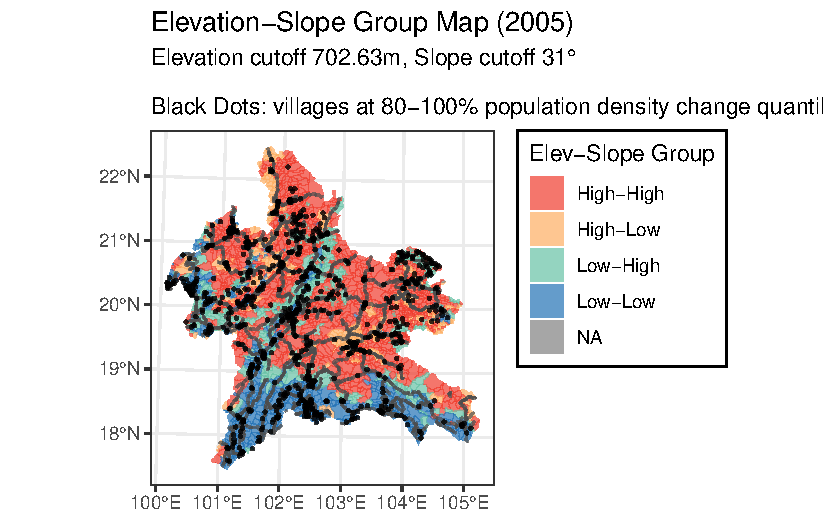
\includegraphics[keepaspectratio]{population_files/figure-pdf/unnamed-chunk-20-1.pdf}}

\pandocbounded{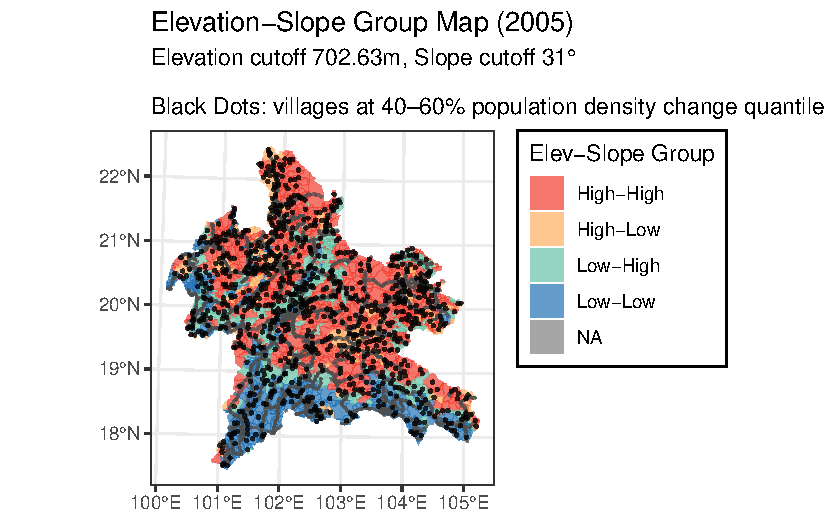
\includegraphics[keepaspectratio]{population_files/figure-pdf/unnamed-chunk-22-1.pdf}}

\pandocbounded{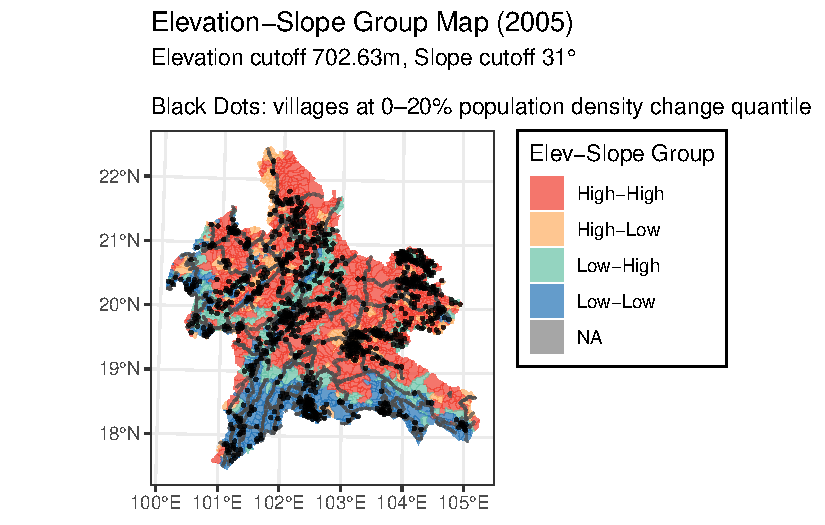
\includegraphics[keepaspectratio]{population_files/figure-pdf/unnamed-chunk-24-1.pdf}}

\begin{longtable}[]{@{}cccccc@{}}
\caption{Number of Villages by Elevation-Slope Group and Population
Density Change Quantile}\tabularnewline
\toprule\noalign{}
elevation\_slope\_group & 0--20\% & 20--40\% & 40--60\% & 60--80\% &
80--100\% \\
\midrule\noalign{}
\endfirsthead
\toprule\noalign{}
elevation\_slope\_group & 0--20\% & 20--40\% & 40--60\% & 60--80\% &
80--100\% \\
\midrule\noalign{}
\endhead
\bottomrule\noalign{}
\endlastfoot
High-High & 228 & 450 & 438 & 369 & 198 \\
High-Low & 162 & 135 & 161 & 155 & 122 \\
Low-High & 201 & 189 & 155 & 109 & 82 \\
Low-Low & 377 & 194 & 214 & 334 & 565 \\
NA & 0 & 0 & 0 & 1 & 0 \\
\end{longtable}

\pandocbounded{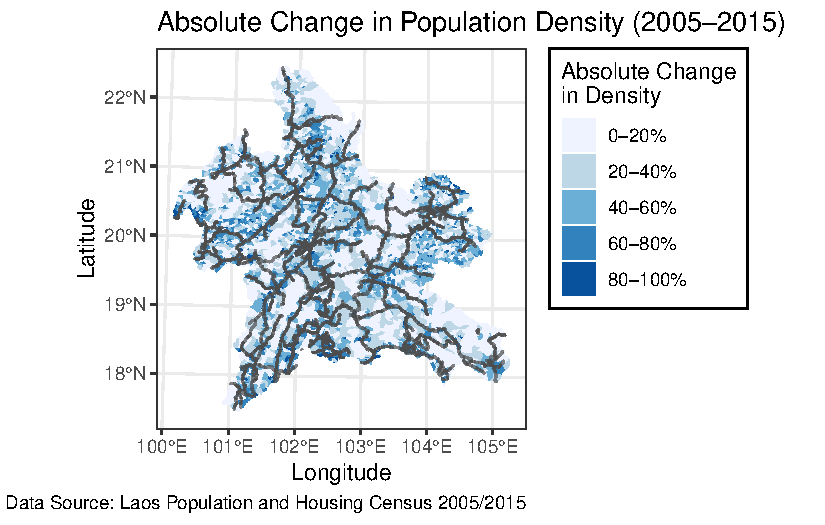
\includegraphics[keepaspectratio]{population_files/figure-pdf/unnamed-chunk-26-1.pdf}}

\begin{itemize}
\item
  \textbf{Population and density changes showed spatial clustering}

  \begin{itemize}
  \tightlist
  \item
    It can be observed that villages that are in the highest quantile
    are also surrounded by villages in lower quantile. In other words,
    villages that experienced higher population density increase are
    close to villages that experienced lower population density
    increase.
  \end{itemize}
\end{itemize}

\begin{longtable}[]{@{}ccccc@{}}
\caption{Summary Statistics of Population Density Change by Quantile
(Census)}\tabularnewline
\toprule\noalign{}
change\_quantile & mean\_val & median\_val & minimum & maximum \\
\midrule\noalign{}
\endfirsthead
\toprule\noalign{}
change\_quantile & mean\_val & median\_val & minimum & maximum \\
\midrule\noalign{}
\endhead
\bottomrule\noalign{}
\endlastfoot
0--20\% & -52.369684 & -14.347769 & -4376.7847000 & -6.0999966 \\
20--40\% & -2.316047 & -2.082729 & -6.0988216 & 0.4348898 \\
40--60\% & 3.700253 & 3.443567 & 0.4367409 & 7.9297333 \\
60--80\% & 17.080334 & 15.665905 & 7.9355316 & 32.0619580 \\
80--100\% & 493.816808 & 84.209671 & 32.1726000 & 19378.7730000 \\
\end{longtable}

From the above table, we can further observe that most of villages in
lower 40\% quantile experience decrease in population density.

\pandocbounded{\includegraphics[keepaspectratio]{population_files/figure-pdf/unnamed-chunk-28-1.pdf}}

\begin{longtable}[]{@{}cccccccc@{}}
\caption{Summary Statistics of Population Change by Elevation Slope
Group (Census Matched)}\tabularnewline
\toprule\noalign{}
elevation\_slope\_group & mean\_c\_population & median\_c\_population &
sd\_c\_population & mean\_g\_population & median\_g\_population &
sd\_g\_population & n \\
\midrule\noalign{}
\endfirsthead
\toprule\noalign{}
elevation\_slope\_group & mean\_c\_population & median\_c\_population &
sd\_c\_population & mean\_g\_population & median\_g\_population &
sd\_g\_population & n \\
\midrule\noalign{}
\endhead
\bottomrule\noalign{}
\endlastfoot
High-High & 118.7104 & 56 & 309.5695 & 0.4909082 & 0.1757720 & 1.194635
& 1913 \\
High-Low & 134.3322 & 54 & 349.5559 & 0.5063868 & 0.1531323 & 1.254268 &
861 \\
Low-High & 120.4988 & 26 & 328.6131 & 0.4934685 & 0.0742074 & 1.426292 &
864 \\
Low-Low & 301.4241 & 114 & 560.9786 & 0.7401963 & 0.2085106 & 1.548728 &
1917 \\
\end{longtable}

Using matched Population and Housing Census dataset, we can observe
villages in low-low elevation-slope group experience higher population
change and higher population growth rate compared to other
elevation-slope group.

\begin{verbatim}
Warning: Using `size` aesthetic for lines was deprecated in ggplot2 3.4.0.
i Please use `linewidth` instead.
\end{verbatim}

\pandocbounded{\includegraphics[keepaspectratio]{population_files/figure-pdf/unnamed-chunk-30-1.pdf}}

\pandocbounded{\includegraphics[keepaspectratio]{population_files/figure-pdf/unnamed-chunk-31-1.pdf}}

Using WorldPop Population Count data, we can also observe that low-low
elevation-slope group have both higher population and population growth
rate compared to high-high group.

\subsubsection{Summary}\label{summary-1}

\textbf{We can conclude that topographic conditions (in our case
elevation and slope) correlate with population dynamics (or how
population change). While there is a `'linear'\,' relationship between
population distribution and topographic characteristics, population
dynamic differ across elevation-slope group class before and after
intervention. To be more specific, low-low elevation-slope group class
might have more drastic population change (both increase and decrease)
while others might face less drastic change.}

\section{Risk Area and Population}\label{risk-area-and-population}

We pointed out that topographic conditions might have different
population distribution and population dynamics. To be more specific,
we've seen that regions with elevation below 700 m AND slope lower than
30° tend to have more population and higher population growth. Note that
the topographic cutoff (700 m elevation and 30° slope) are selected
without any specific criteria but coincided with topographic condition
suitable for opium poppy cultivation. In this section, we further
manipulate this cutoff based on our definition of risk area and see
whether risk area has different population distribution and dynamic
(population growth) compared to non-risk area.

Recall that our definition of risk area contains the following:

\begin{enumerate}
\def\labelenumi{\alph{enumi}.}
\tightlist
\item
  Regions with elevation between 700 \textasciitilde{} 2000 meters
  (UNODC 2001);
\item
  Regions with Slope between 20° to 40° (Administration et al. 1992);
\item
  Regions with recorded opium cultivation nearby during 2000 nation wide
  opium survey (UNODC 2000)
\end{enumerate}

Raster cells that matches the above condition are considered as risk
cell. Risk level for each village/district/province are computed using
the following formula:

\[
\textrm{Risk Level} = \frac{(\textrm{# of Risk Cell} \times 100 \times 100) / 1000000}{\textrm{Area of Village/District/Province in Square Kilometer}}
\] Risk Level we defined using the above formula represents that
percentage of total area of village/district/province that is vulnerable
to opium poppy cultivation based on topographic suitability and
historical cultivation.

We attempt to answer following questions:

\begin{enumerate}
\def\labelenumi{\arabic{enumi}.}
\tightlist
\item
  Does villages in risk area experience different population growth
  compared to villages not in risk area? Do villages with higher risk
  level experience different population growth compared to villages with
  lower risk level?
\item
  What is the relationship between risk area and establishment of ORP
  program?
\item
  Does villages in risk area AND higher exposure to ORP experience
  different population growth compared to villages in risk area but has
  lower exposure to ORP?
\end{enumerate}

\subsection{Population Growth Comparison by Risk
Level}\label{population-growth-comparison-by-risk-level}

In this section, we will compare the population growth between risk area
and non-risk area at village/district/province level. We will first
compare with risk level using continuous measure. Then, we will
construct a binary variable by setting a threshold to determine whether
it belongs to risk area or non-risk area.

\subsubsection{Village Level Population Growth
Comparison}\label{village-level-population-growth-comparison}

\begin{Shaded}
\begin{Highlighting}[]
\CommentTok{\# Fit linear model}
\NormalTok{model\_1 }\OtherTok{\textless{}{-}} \FunctionTok{lm}\NormalTok{(g\_population }\SpecialCharTok{\textasciitilde{}}\NormalTok{ risk\_level, }\AttributeTok{data =}\NormalTok{ matched\_0515)}
\NormalTok{summary\_1 }\OtherTok{\textless{}{-}} \FunctionTok{summary}\NormalTok{(model\_1)}

\CommentTok{\# Extract values}
\NormalTok{coef\_1 }\OtherTok{\textless{}{-}}\NormalTok{ summary\_1}\SpecialCharTok{$}\NormalTok{coefficients[}\StringTok{"risk\_level"}\NormalTok{, }\StringTok{"Estimate"}\NormalTok{]}
\NormalTok{se\_1   }\OtherTok{\textless{}{-}}\NormalTok{ summary\_1}\SpecialCharTok{$}\NormalTok{coefficients[}\StringTok{"risk\_level"}\NormalTok{, }\StringTok{"Std. Error"}\NormalTok{]}
\NormalTok{r2\_1   }\OtherTok{\textless{}{-}}\NormalTok{ summary\_1}\SpecialCharTok{$}\NormalTok{r.squared}

\CommentTok{\# Format label}
\NormalTok{label\_1 }\OtherTok{\textless{}{-}} \FunctionTok{sprintf}\NormalTok{(}\StringTok{"β = \%.3f (SE = \%.3f)}\SpecialCharTok{\textbackslash{}n}\StringTok{R² = \%.3f"}\NormalTok{, coef\_1, se\_1, r2\_1)}

\CommentTok{\# Plot}
\NormalTok{p1 }\OtherTok{\textless{}{-}} \FunctionTok{ggplot}\NormalTok{(matched\_0515, }\FunctionTok{aes}\NormalTok{(}\AttributeTok{x =}\NormalTok{ risk\_level, }\AttributeTok{y =}\NormalTok{ g\_population)) }\SpecialCharTok{+}
  \FunctionTok{geom\_point}\NormalTok{(}\AttributeTok{alpha =} \FloatTok{0.5}\NormalTok{) }\SpecialCharTok{+}
  \FunctionTok{geom\_smooth}\NormalTok{(}\AttributeTok{method =} \StringTok{"lm"}\NormalTok{, }\AttributeTok{color =} \StringTok{"blue"}\NormalTok{, }\AttributeTok{se =} \ConstantTok{TRUE}\NormalTok{) }\SpecialCharTok{+}
  \FunctionTok{annotate}\NormalTok{(}\StringTok{"text"}\NormalTok{, }\AttributeTok{x =} \ConstantTok{Inf}\NormalTok{, }\AttributeTok{y =} \ConstantTok{Inf}\NormalTok{, }\AttributeTok{label =}\NormalTok{ label\_1, }\AttributeTok{hjust =} \FloatTok{1.1}\NormalTok{, }\AttributeTok{vjust =} \FloatTok{1.5}\NormalTok{, }\AttributeTok{size =} \DecValTok{5}\NormalTok{) }\SpecialCharTok{+}
  \FunctionTok{labs}\NormalTok{(}
    \AttributeTok{x =} \StringTok{"Village Risk Level"}\NormalTok{,}
    \AttributeTok{y =} \StringTok{"Population Growth Rate"}
\NormalTok{  ) }\SpecialCharTok{+}
  \FunctionTok{theme\_bw}\NormalTok{()}

\CommentTok{\# Fit linear model}
\NormalTok{model\_1 }\OtherTok{\textless{}{-}} \FunctionTok{lm}\NormalTok{(g\_population }\SpecialCharTok{\textasciitilde{}}\NormalTok{ risk\_binary, }\AttributeTok{data =}\NormalTok{ matched\_0515)}
\NormalTok{summary\_1 }\OtherTok{\textless{}{-}} \FunctionTok{summary}\NormalTok{(model\_1)}

\CommentTok{\# Extract values}
\NormalTok{coef\_1 }\OtherTok{\textless{}{-}}\NormalTok{ summary\_1}\SpecialCharTok{$}\NormalTok{coefficients[}\StringTok{"risk\_binaryRisk"}\NormalTok{, }\StringTok{"Estimate"}\NormalTok{]}
\NormalTok{se\_1   }\OtherTok{\textless{}{-}}\NormalTok{ summary\_1}\SpecialCharTok{$}\NormalTok{coefficients[}\StringTok{"risk\_binaryRisk"}\NormalTok{, }\StringTok{"Std. Error"}\NormalTok{]}
\NormalTok{r2\_1   }\OtherTok{\textless{}{-}}\NormalTok{ summary\_1}\SpecialCharTok{$}\NormalTok{r.squared}

\CommentTok{\# Format label}
\NormalTok{label\_1 }\OtherTok{\textless{}{-}} \FunctionTok{sprintf}\NormalTok{(}\StringTok{"β = \%.3f (SE = \%.3f)}\SpecialCharTok{\textbackslash{}n}\StringTok{R² = \%.3f"}\NormalTok{, coef\_1, se\_1, r2\_1)}

\CommentTok{\# Plot}
\NormalTok{p2 }\OtherTok{\textless{}{-}} \FunctionTok{ggplot}\NormalTok{(matched\_0515, }\FunctionTok{aes}\NormalTok{(}\AttributeTok{x =}\NormalTok{ risk\_binary, }\AttributeTok{y =}\NormalTok{ g\_population)) }\SpecialCharTok{+}
  \FunctionTok{geom\_boxplot}\NormalTok{() }\SpecialCharTok{+}
  \FunctionTok{annotate}\NormalTok{(}\StringTok{"text"}\NormalTok{, }\AttributeTok{x =} \ConstantTok{Inf}\NormalTok{, }\AttributeTok{y =} \ConstantTok{Inf}\NormalTok{, }\AttributeTok{label =}\NormalTok{ label\_1, }\AttributeTok{hjust =} \FloatTok{1.1}\NormalTok{, }\AttributeTok{vjust =} \FloatTok{1.5}\NormalTok{, }\AttributeTok{size =} \DecValTok{5}\NormalTok{) }\SpecialCharTok{+}
  \FunctionTok{labs}\NormalTok{(}
    \AttributeTok{x =} \FunctionTok{sprintf}\NormalTok{(}\StringTok{"Village Risk Level (Binary: Threshold = \%.2f)"}\NormalTok{, risk\_threshold),}
    \AttributeTok{y =} \StringTok{"Population Growth Rate"}
\NormalTok{  ) }\SpecialCharTok{+}
  \FunctionTok{coord\_cartesian}\NormalTok{(}\AttributeTok{ylim =} \FunctionTok{c}\NormalTok{(}\SpecialCharTok{{-}}\DecValTok{1}\NormalTok{, }\DecValTok{1}\NormalTok{)) }\SpecialCharTok{+}
  \FunctionTok{theme\_bw}\NormalTok{()}

\NormalTok{(p1 }\SpecialCharTok{+}\NormalTok{ p2) }\SpecialCharTok{+} 
  \FunctionTok{plot\_annotation}\NormalTok{(}
    \AttributeTok{title =} \StringTok{"Village Risk Level and Population Growth Rate"}\NormalTok{,}
    \AttributeTok{theme =} \FunctionTok{theme}\NormalTok{(}\AttributeTok{plot.title =} \FunctionTok{element\_text}\NormalTok{(}\AttributeTok{size =} \DecValTok{14}\NormalTok{, }\AttributeTok{face =} \StringTok{"bold"}\NormalTok{, }\AttributeTok{hjust =} \FloatTok{0.5}\NormalTok{))}
\NormalTok{  )}
\end{Highlighting}
\end{Shaded}

\begin{verbatim}
`geom_smooth()` using formula = 'y ~ x'
\end{verbatim}

\pandocbounded{\includegraphics[keepaspectratio]{population_files/figure-pdf/unnamed-chunk-33-1.pdf}}

As show in the above figure, we can see that there's a negative
correlation between village population growth rate and village risk
level. This indicates that villages with higher opium cultivation risk
level tend to have lower population growth rate.

\pandocbounded{\includegraphics[keepaspectratio]{population_files/figure-pdf/unnamed-chunk-34-1.pdf}}

\subsubsection{District Level Population Growth
Comparison}\label{district-level-population-growth-comparison}

\begin{verbatim}
`geom_smooth()` using formula = 'y ~ x'
\end{verbatim}

\pandocbounded{\includegraphics[keepaspectratio]{population_files/figure-pdf/unnamed-chunk-35-1.pdf}}

At the district level, it becomes more obvious (indicated by steeper
negative slope) that district with higher risk level tend to have lower
population growth rate.

\pandocbounded{\includegraphics[keepaspectratio]{population_files/figure-pdf/unnamed-chunk-36-1.pdf}}

\subsubsection{Province Level Population Growth
Comparison}\label{province-level-population-growth-comparison}

\begin{verbatim}
`geom_smooth()` using formula = 'y ~ x'
\end{verbatim}

\pandocbounded{\includegraphics[keepaspectratio]{population_files/figure-pdf/unnamed-chunk-37-1.pdf}}

At the province level, it becomes more obvious (indicated by steeper
negative slope) that province with higher risk level tend to have lower
population growth rate.

\pandocbounded{\includegraphics[keepaspectratio]{population_files/figure-pdf/unnamed-chunk-38-1.pdf}}

\section{Risk Area and ORP}\label{risk-area-and-orp}

In this section, we check whether ORP programs are established where the
opium cultivation risk is higher as the purpose of ORP suggest by using
official ORP records (district/province level) and risk level variable
we constructed above.

\begin{verbatim}
`geom_smooth()` using formula = 'y ~ x'
\end{verbatim}

\pandocbounded{\includegraphics[keepaspectratio]{population_files/figure-pdf/unnamed-chunk-40-1.pdf}}

As shown in the figure above, we can see that there's a positive
correlation between number of ORP program within the district and
district's risk level, indicating that number of ORP tend to be high
where districts are suitable for opium cultivation or historically
cultivated opium poppy.

\begin{verbatim}
`geom_smooth()` using formula = 'y ~ x'
\end{verbatim}

\pandocbounded{\includegraphics[keepaspectratio]{population_files/figure-pdf/unnamed-chunk-41-1.pdf}}

At the province level, there seems to be positive correlation between
province risk level and number of ORP programs within province. However,
the relationship is not statistically significant.

\section{ORP and Topographic
Conditions}\label{orp-and-topographic-conditions}

We want to characterize location where ORP is likely to be established
using topographic condition rather than using ORP records directly since
there might be endogeneity issue. That is, ORP alternative crop
plantation might be established where labor force is abundant while
population might also react if the ORP alternative crop plantation is
established nearby.

In previous section, we pointed out that topographic conditions might
have different population distribution and population dynamics
(population growth). In this section, we further classify the
topographic condition that is more likely to attract ORP alternative
crop plantation.

Since the topographic conditions might determine the baseline population
distribution and the population dynamic across years, we anticipate that
ORP might also have differential impact on different elevation-slope
group. In this section, we evaluate the following:

\begin{enumerate}
\def\labelenumi{\arabic{enumi}.}
\tightlist
\item
  Controlling for topographic conditions, do provinces and districts
  that have ORP nearby experience different population growth compared
  to those without any ORP program nearby?
\item
  Controlling for topographic conditions, do provinces and districts
  that have more ORP program/higher ORP intensity experience different
  population growth compared to those that have less ORP program/lower
  ORP intensity?
\item
  Controlling for topographic conditions, do villages with opium
  cultivation risk experience different population growth compared to
  those with no opium cultivation risk?
\item
  Controlling for topographic conditions, do villages with higher opium
  cultivation risk experience different population growth compared to
  those with lower opium cultivation risk?
\item
  Controlling for topographic conditions, do provinces and districts
  with ORP program nearby and opium cultivation risk experience
  different population growth compared to those that have no ORP program
  nearby and no opium cultivation risk.
\item
  Controlling for topographic conditions, do provinces and districts
  with more ORP program/higher ORP intensity and higher opium
  cultivation risk experience different population growth compared to
  those with less ORP program/lower ORP intensity and with lower opium
  cultivation risk.
\end{enumerate}

\subsection{Elevation-Slope Group}\label{elevation-slope-group}

From above observation, we've seen that low-low elevation-slope class
tend to have higher population compared to high-high and other
elevation-slope class. In this section, we'll look further into the
population distribution and dynamics by comparing different
elevation-slope class.

\begin{longtable}[]{@{}ccccc@{}}
\caption{Summary Statistics of Population by Elevation-Slope Group
(Census) in 2005}\tabularnewline
\toprule\noalign{}
elevation\_slope\_group & n\_village & n\_population & mean\_population
& sd\_population \\
\midrule\noalign{}
\endfirsthead
\toprule\noalign{}
elevation\_slope\_group & n\_village & n\_population & mean\_population
& sd\_population \\
\midrule\noalign{}
\endhead
\bottomrule\noalign{}
\endlastfoot
High-High & 1915 & 687363 & 358.9363 & 238.7187 \\
High-Low & 863 & 373327 & 432.5921 & 360.5670 \\
Low-High & 865 & 323155 & 373.5896 & 239.7567 \\
Low-Low & 1918 & 1231830 & 642.2471 & 447.7559 \\
NA & 5 & 1499 & 299.8000 & 172.7808 \\
\end{longtable}

\begin{longtable}[]{@{}ccccc@{}}
\caption{Summary Statistics of Population by Elevation-Slope Group
(Census) in 2015}\tabularnewline
\toprule\noalign{}
elevation\_slope\_group & n\_village & n\_population & mean\_population
& sd\_population \\
\midrule\noalign{}
\endfirsthead
\toprule\noalign{}
elevation\_slope\_group & n\_village & n\_population & mean\_population
& sd\_population \\
\midrule\noalign{}
\endhead
\bottomrule\noalign{}
\endlastfoot
High-High & 1683 & 774542 & 460.2151 & 373.8352 \\
High-Low & 735 & 398841 & 542.6408 & 478.9906 \\
Low-High & 736 & 338928 & 460.5000 & 344.7111 \\
Low-Low & 1684 & 1452467 & 862.5101 & 666.8117 \\
NA & 1 & 560 & 560.0000 & NA \\
\end{longtable}

From the table above we can see low-low elevation-slope class has higher
mean village population followed by high-low, low-high, and high-high
class. We can also observe the mean village population difference
between high-high and low-low elevation-slope class is 283 in 2005 and
the gap increased into 418 in 2015.

\begin{verbatim}
Warning: Removed 4 rows containing non-finite outside the scale range
(`stat_density()`).
\end{verbatim}

\begin{verbatim}
Warning: Removed 38 rows containing non-finite outside the scale range
(`stat_density()`).
\end{verbatim}

\begin{verbatim}
Warning: Groups with fewer than two data points have been dropped.
\end{verbatim}

\begin{verbatim}
Warning in max(ids, na.rm = TRUE): no non-missing arguments to max; returning
-Inf
\end{verbatim}

\pandocbounded{\includegraphics[keepaspectratio]{population_files/figure-pdf/unnamed-chunk-43-1.pdf}}

\begin{Shaded}
\begin{Highlighting}[]
\CommentTok{\# Shared y{-}axis limit}
\NormalTok{y\_lim }\OtherTok{\textless{}{-}} \FunctionTok{c}\NormalTok{(}\DecValTok{0}\NormalTok{, }\DecValTok{3000}\NormalTok{)}

\CommentTok{\# Boxplot for 2005}
\NormalTok{p1 }\OtherTok{\textless{}{-}} \FunctionTok{ggplot}\NormalTok{(v\_2005,}
             \FunctionTok{aes}\NormalTok{(}\AttributeTok{x =}\NormalTok{ elevation\_slope\_group, }\AttributeTok{y =}\NormalTok{ population, }\AttributeTok{fill =}\NormalTok{ elevation\_slope\_group)) }\SpecialCharTok{+}
  \FunctionTok{geom\_boxplot}\NormalTok{(}\AttributeTok{outlier.alpha =} \FloatTok{0.2}\NormalTok{, }\AttributeTok{width =} \FloatTok{0.5}\NormalTok{) }\SpecialCharTok{+}
  \FunctionTok{scale\_y\_continuous}\NormalTok{(}\AttributeTok{limits =}\NormalTok{ y\_lim) }\SpecialCharTok{+}
  \FunctionTok{labs}\NormalTok{(}
    \AttributeTok{title =} \StringTok{"Population by Elevation{-}Slope Group (2005)"}\NormalTok{,}
    \AttributeTok{x =} \ConstantTok{NULL}\NormalTok{,}
    \AttributeTok{y =} \StringTok{"Village Population"}\NormalTok{,}
    \AttributeTok{fill =} \StringTok{"Elevation{-}Slope Group"}
\NormalTok{  ) }\SpecialCharTok{+}
  \FunctionTok{theme\_bw}\NormalTok{() }\SpecialCharTok{+}
  \FunctionTok{theme}\NormalTok{(}\AttributeTok{legend.position =} \StringTok{"none"}\NormalTok{)}

\CommentTok{\# Boxplot for 2015}
\NormalTok{p2 }\OtherTok{\textless{}{-}} \FunctionTok{ggplot}\NormalTok{(v\_2015,}
             \FunctionTok{aes}\NormalTok{(}\AttributeTok{x =}\NormalTok{ elevation\_slope\_group, }\AttributeTok{y =}\NormalTok{ population, }\AttributeTok{fill =}\NormalTok{ elevation\_slope\_group)) }\SpecialCharTok{+}
  \FunctionTok{geom\_boxplot}\NormalTok{(}\AttributeTok{outlier.alpha =} \FloatTok{0.2}\NormalTok{, }\AttributeTok{width =} \FloatTok{0.5}\NormalTok{) }\SpecialCharTok{+}
  \FunctionTok{scale\_y\_continuous}\NormalTok{(}\AttributeTok{limits =}\NormalTok{ y\_lim) }\SpecialCharTok{+}
  \FunctionTok{labs}\NormalTok{(}
    \AttributeTok{title =} \StringTok{"Population by Elevation{-}Slope Group (2015)"}\NormalTok{,}
    \AttributeTok{x =} \ConstantTok{NULL}\NormalTok{,}
    \AttributeTok{y =} \StringTok{"Village Population"}\NormalTok{,}
    \AttributeTok{fill =} \StringTok{"Elevation{-}Slope Group"}
\NormalTok{  ) }\SpecialCharTok{+}
  \FunctionTok{theme\_bw}\NormalTok{() }\SpecialCharTok{+}
  \FunctionTok{theme}\NormalTok{(}\AttributeTok{legend.position =} \StringTok{"none"}\NormalTok{)}

\CommentTok{\# Combine plots side{-}by{-}side}
\NormalTok{p1 }\SpecialCharTok{+}\NormalTok{ p2 }\SpecialCharTok{+} \FunctionTok{plot\_layout}\NormalTok{(}\AttributeTok{guides =} \StringTok{"collect"}\NormalTok{) }\SpecialCharTok{\&} \FunctionTok{theme}\NormalTok{(}\AttributeTok{legend.position =} \StringTok{"bottom"}\NormalTok{)}
\end{Highlighting}
\end{Shaded}

\begin{verbatim}
Warning: Removed 4 rows containing non-finite outside the scale range
(`stat_boxplot()`).
\end{verbatim}

\begin{verbatim}
Warning: Removed 38 rows containing non-finite outside the scale range
(`stat_boxplot()`).
\end{verbatim}

\pandocbounded{\includegraphics[keepaspectratio]{population_files/figure-pdf/unnamed-chunk-44-1.pdf}}

\subsection{ORP Programs}\label{orp-programs}

\begin{verbatim}
`summarise()` has grouped output by 'PCODE'. You can override using the
`.groups` argument.
\end{verbatim}

\begin{longtable}[]{@{}ccccc@{}}
\caption{Province Level ORP program and Population
(2005)}\tabularnewline
\toprule\noalign{}
PCODE & PNAME & total\_pop & mean\_pop & n\_prov\_proj \\
\midrule\noalign{}
\endfirsthead
\toprule\noalign{}
PCODE & PNAME & total\_pop & mean\_pop & n\_prov\_proj \\
\midrule\noalign{}
\endhead
\bottomrule\noalign{}
\endlastfoot
2 & Phongsaly & 222721 & 267.6935 & 171 \\
3 & Luangnamtha & 201913 & 367.7832 & 298 \\
4 & Oudomxay & 435107 & 432.9423 & 208 \\
5 & Bokeo & 209445 & 378.0596 & 298 \\
6 & Luangprabang & 632355 & 449.4350 & 171 \\
7 & Huaphanh & 372936 & 348.5383 & NA \\
8 & Xayaboury & 550035 & 661.0998 & 208 \\
9 & Xiengkhuang & 372871 & 407.5093 & NA \\
10 & Vientiane & 819282 & 666.0829 & 55 \\
11 & Borikhamxay & 327924 & 686.0335 & NA \\
\end{longtable}

\begin{verbatim}
`summarise()` has grouped output by 'PCODE'. You can override using the
`.groups` argument.
\end{verbatim}

\begin{longtable}[]{@{}ccccc@{}}
\caption{Province Level ORP program and Population
(2015)}\tabularnewline
\toprule\noalign{}
PCODE & PNAME & total\_pop & mean\_pop & n\_prov\_proj \\
\midrule\noalign{}
\endfirsthead
\toprule\noalign{}
PCODE & PNAME & total\_pop & mean\_pop & n\_prov\_proj \\
\midrule\noalign{}
\endhead
\bottomrule\noalign{}
\endlastfoot
2 & Phongsaly & 229090 & 320.4056 & 171 \\
3 & Louangnamtha & 243367 & 464.4408 & 298 \\
4 & Oudomxai & 507693 & 584.2267 & 171 \\
5 & Bokeo & 277017 & 653.3420 & 298 \\
6 & Louangphabang & 693029 & 543.1262 & 171 \\
7 & Houaphan & 397752 & 405.8694 & NA \\
8 & Xaignabouly & 637876 & 840.4163 & 208 \\
9 & Xiengkhouang & 371510 & 482.4805 & NA \\
10 & Vientiane & 818823 & 997.3484 & 55 \\
11 & Bolikhamxai & 394383 & 864.8750 & NA \\
18 & Xaisomboun & 234205 & 791.2331 & 55 \\
\end{longtable}

\begin{longtable}[]{@{}ccccccc@{}}
\caption{Province Level ORP program and Population (2005
\textasciitilde{} 2015)}\tabularnewline
\toprule\noalign{}
PCODE & PNAME & mean\_pop\_2005 & mean\_pop\_2015 & diff\_mean\_pop &
p\_value & n\_prov\_proj \\
\midrule\noalign{}
\endfirsthead
\toprule\noalign{}
PCODE & PNAME & mean\_pop\_2005 & mean\_pop\_2015 & diff\_mean\_pop &
p\_value & n\_prov\_proj \\
\midrule\noalign{}
\endhead
\bottomrule\noalign{}
\endlastfoot
2 & Phongsaly & 267.6935 & 320.4056 & 52.71208 & 2.00e-07 & 171 \\
3 & Luangnamtha & 367.7832 & 464.4408 & 96.65760 & 2.00e-07 & 298 \\
4 & Oudomxay & 432.9423 & 584.2267 & 151.28441 & 0.00e+00 & 208 \\
6 & Luangprabang & 449.4350 & 543.1262 & 93.69121 & 0.00e+00 & 171 \\
7 & Huaphanh & 348.5383 & 405.8694 & 57.33107 & 7.10e-06 & 0 \\
5 & Bokeo & 378.0596 & 653.3420 & 275.28241 & 0.00e+00 & 298 \\
9 & Xiengkhuang & 407.5093 & 482.4805 & 74.97123 & 2.83e-05 & 0 \\
8 & Xayaboury & 661.0998 & 840.4163 & 179.31658 & 0.00e+00 & 208 \\
10 & Vientiane & 666.0829 & 997.3484 & 331.26543 & 0.00e+00 & 55 \\
11 & Borikhamxay & 686.0335 & 864.8750 & 178.84153 & 6.50e-06 & 0 \\
\end{longtable}

\begin{verbatim}
`geom_smooth()` using formula = 'y ~ x'
\end{verbatim}

\pandocbounded{\includegraphics[keepaspectratio]{population_files/figure-pdf/unnamed-chunk-48-1.pdf}}

\begin{verbatim}
`geom_smooth()` using formula = 'y ~ x'
\end{verbatim}

\pandocbounded{\includegraphics[keepaspectratio]{population_files/figure-pdf/unnamed-chunk-48-2.pdf}}

\begin{verbatim}
`summarise()` has grouped output by 'DCODE'. You can override using the
`.groups` argument.
\end{verbatim}

\begin{longtable}[]{@{}ccccc@{}}
\caption{District Level ORP program and Population
(2005)}\tabularnewline
\toprule\noalign{}
DCODE & DNAME & total\_pop & mean\_pop & n\_dist\_proj \\
\midrule\noalign{}
\endfirsthead
\toprule\noalign{}
DCODE & DNAME & total\_pop & mean\_pop & n\_dist\_proj \\
\midrule\noalign{}
\endhead
\bottomrule\noalign{}
\endlastfoot
201 & Phongsaly & 30598 & 259.3051 & 18 \\
202 & May & 31100 & 246.8254 & 4 \\
203 & Khua & 47123 & 237.9949 & 21 \\
204 & Samphanh & 37455 & 312.1250 & 18 \\
205 & Boon neua & 22195 & 270.6707 & 25 \\
206 & Nhot ou & 29141 & 297.3571 & 36 \\
207 & Boontai & 25109 & 278.9889 & 18 \\
301 & Namtha & 57590 & 509.6460 & 36 \\
302 & Sing & 32527 & 315.7961 & 54 \\
303 & Long & 36531 & 344.6321 & 54 \\
304 & Viengphoukha & 33944 & 440.8312 & 36 \\
305 & Nalae & 41321 & 275.4733 & 27 \\
401 & Xay & 89880 & 554.8148 & 49 \\
402 & La & 30180 & 382.0253 & 38 \\
403 & Namor & 51947 & 396.5420 & 29 \\
404 & Nga & 63189 & 394.9312 & 49 \\
405 & Beng & 51946 & 535.5258 & 49 \\
406 & Hoon & 84527 & 396.8404 & 27 \\
407 & Parkbeng & 63438 & 389.1902 & NA \\
501 & Huoixai & 67128 & 422.1887 & 19 \\
502 & Tonpheung & 28101 & 432.3231 & 2 \\
503 & Meung & 19134 & 341.6786 & 73 \\
504 & Pha oudom & 60638 & 342.5876 & 19 \\
505 & Paktha & 34444 & 355.0928 & 19 \\
601 & Luangprabang & 107625 & 656.2500 & 2 \\
602 & Xieng ngeun & 49052 & 426.5391 & 2 \\
603 & Nan & 55376 & 419.5152 & 2 \\
604 & Park ou & 34116 & 396.6977 & 8 \\
605 & Nambak & 93526 & 560.0359 & 14 \\
606 & Ngoi & 58394 & 347.5833 & 4 \\
607 & Pak xeng & 36208 & 362.0800 & NA \\
608 & Phonxay & 47046 & 448.0571 & NA \\
609 & Chomphet & 51918 & 439.9831 & NA \\
610 & Viengkham & 62865 & 390.4658 & NA \\
611 & Phoukhoune & 36229 & 398.1209 & 3 \\
701 & Xamneua & 66160 & 501.2121 & NA \\
702 & Xiengkhor & 35327 & 447.1772 & NA \\
703 & Viengthong & 50198 & 334.6533 & NA \\
704 & Viengxay & 41079 & 268.4902 & NA \\
705 & Huameuang & 46492 & 309.9467 & NA \\
706 & Xamtay & 71173 & 309.4478 & NA \\
707 & Sopbao & 30882 & 372.0723 & NA \\
708 & Add & 31625 & 340.0538 & NA \\
801 & Xayaboury & 116398 & 619.1383 & 2 \\
802 & Khop & 37312 & 678.4000 & NA \\
803 & Hongsa & 52455 & 468.3482 & NA \\
804 & Ngeun & 27425 & 583.5106 & NA \\
805 & Xienghone & 42105 & 628.4328 & NA \\
806 & Phiang & 59369 & 836.1831 & 3 \\
807 & Parklai & 126244 & 864.6849 & NA \\
808 & Kenethao & 53367 & 620.5465 & 2 \\
809 & Botene & 23466 & 586.6500 & NA \\
810 & Thongmyxay & 11894 & 594.7000 & 16 \\
901 & Pek & 80844 & 581.6115 & NA \\
902 & Kham & 69584 & 353.2183 & NA \\
903 & Nonghed & 48152 & 341.5035 & NA \\
904 & Khoune & 42978 & 330.6000 & NA \\
905 & Mokmai & 23550 & 392.5000 & NA \\
906 & Phookood & 61417 & 584.9238 & NA \\
907 & Phaxay & 19840 & 300.6061 & NA \\
908 & Thathom & 26506 & 344.2338 & NA \\
1001 & Phonhong & 95041 & 766.4597 & NA \\
1002 & Thoulakhom & 128579 & 840.3856 & 3 \\
1003 & Keo oudom & 31728 & 537.7627 & 5 \\
1004 & Kasy & 48511 & 411.1102 & 4 \\
1005 & Vangvieng & 79976 & 605.8788 & 5 \\
1006 & Feuang & 55875 & 745.0000 & 5 \\
1007 & Xanakham & 67254 & 723.1613 & 2 \\
1008 & Mad & 37907 & 412.0326 & NA \\
1009 & Viengkham & 37134 & 1092.1765 & NA \\
1010 & Hinheup & 48194 & 634.1316 & 5 \\
1011 & Hom & 58760 & 462.6772 & NA \\
1012 & Xaysomboon & 53740 & 577.8495 & NA \\
1013 & Muen & 76583 & 1418.2037 & 5 \\
1101 & Parkxane & 50575 & 648.3974 & NA \\
1102 & Thaphabath & 72450 & 832.7586 & NA \\
1103 & Pakkading & 45431 & 770.0169 & NA \\
1104 & Bolikhanh & 60369 & 628.8438 & NA \\
1105 & Khamkheuth & 68816 & 674.6667 & NA \\
1106 & Viengthong & 30283 & 540.7679 & NA \\
\end{longtable}

\begin{verbatim}
`summarise()` has grouped output by 'DCODE'. You can override using the
`.groups` argument.
\end{verbatim}

\begin{longtable}[]{@{}ccccc@{}}
\caption{District Level ORP program and Population
(2015)}\tabularnewline
\toprule\noalign{}
DCODE & DNAME & total\_pop & mean\_pop & n\_dist\_proj \\
\midrule\noalign{}
\endfirsthead
\toprule\noalign{}
DCODE & DNAME & total\_pop & mean\_pop & n\_dist\_proj \\
\midrule\noalign{}
\endhead
\bottomrule\noalign{}
\endlastfoot
201 & Phongsaly & 27047 & 300.5222 & 18 \\
202 & May & 34074 & 286.3361 & 4 \\
203 & Khua & 42753 & 263.9074 & 4 \\
204 & Samphanh & 32383 & 351.9891 & 18 \\
205 & Boon neua & 26771 & 334.6375 & 25 \\
206 & Nhot ou & 32970 & 392.5000 & 36 \\
207 & Boontai & 33092 & 376.0455 & 21 \\
301 & Namtha & 70377 & 657.7290 & 36 \\
302 & Sing & 43162 & 423.1569 & 54 \\
303 & Long & 41310 & 430.3125 & 54 \\
304 & Viengphoukha & 41211 & 564.5342 & 36 \\
305 & Nalae & 47307 & 324.0205 & 36 \\
401 & Xay & 105910 & 710.8054 & 49 \\
402 & La & 28358 & 333.6235 & 9 \\
403 & Namor & 73649 & 613.7417 & 38 \\
404 & Nga & 74257 & 479.0774 & NA \\
405 & Beng & 55335 & 666.6867 & 49 \\
406 & Hoon & 94326 & 688.5109 & 27 \\
407 & Pakbeng & 75858 & 541.8429 & NA \\
501 & Huoixai & 93444 & 826.9381 & 19 \\
502 & Tonpheung & 38620 & 898.1395 & 2 \\
503 & Meung & 25851 & 550.0213 & 73 \\
504 & Pha oudom & 72459 & 496.2945 & 27 \\
505 & Paktha & 46643 & 621.9067 & 19 \\
601 & Luangprabang & 131285 & 745.9375 & 2 \\
602 & Xieng ngeun & 45063 & 653.0870 & 2 \\
603 & Nan & 53408 & 489.9817 & 2 \\
604 & Park ou & 38012 & 500.1579 & 8 \\
605 & Nambak & 103930 & 742.3571 & 14 \\
606 & Ngoi & 42889 & 363.4661 & 4 \\
607 & Pak xeng & 36715 & 417.2159 & NA \\
608 & Phonxay & 53660 & 536.6000 & NA \\
609 & Chomphet & 52606 & 431.1967 & 10 \\
610 & Viengkham & 51535 & 440.4701 & NA \\
611 & Phoukhoune & 48992 & 576.3765 & 4 \\
612 & Phonthong & 34934 & 459.6579 & 4 \\
701 & Xamneua & 69373 & 502.7029 & NA \\
702 & Xiengkhor & 34035 & 453.8000 & NA \\
703 & Huim & 25970 & 341.7105 & NA \\
704 & Viengxay & 36314 & 307.7458 & NA \\
705 & Huameuang & 63212 & 486.2462 & NA \\
706 & Xamtay & 45874 & 382.2833 & NA \\
707 & Sopbao & 31527 & 389.2222 & NA \\
708 & Add & 29848 & 347.0698 & NA \\
709 & Kuane & 32509 & 369.4205 & NA \\
710 & Sone & 29090 & 427.7941 & NA \\
801 & Xayabury & 121945 & 776.7197 & 2 \\
802 & Khop & 38731 & 730.7736 & NA \\
803 & Hongsa & 61792 & 813.0526 & NA \\
804 & Ngeun & 33812 & 845.3000 & NA \\
805 & Xienghone & 51979 & 775.8060 & NA \\
806 & Phiang & 68780 & 1091.7460 & 16 \\
807 & Parklai & 150841 & 992.3750 & NA \\
808 & Kenethao & 54472 & 801.0588 & 2 \\
809 & Botene & 23754 & 625.1053 & NA \\
810 & Thongmyxay & 10846 & 638.0000 & NA \\
811 & Xaysathan & 20924 & 747.2857 & 8 \\
901 & Pek & 88376 & 640.4058 & NA \\
902 & Kham & 72441 & 476.5855 & NA \\
903 & Nonghed & 54201 & 351.9545 & NA \\
904 & Khoune & 47002 & 427.2909 & NA \\
905 & Morkmay & 25845 & 506.7647 & NA \\
906 & Phoukoud & 63684 & 589.6667 & 3 \\
907 & Phaxay & 19961 & 350.1930 & NA \\
1001 & Phonhong & 106807 & 1057.4950 & NA \\
1002 & Thoulakhom & 157372 & 1513.1923 & 3 \\
1003 & Keo oudom & 30767 & 569.7593 & NA \\
1004 & Kasy & 62835 & 654.5312 & 5 \\
1005 & Vangvieng & 97239 & 892.1009 & 5 \\
1006 & Feuang & 67870 & 998.0882 & 5 \\
1007 & Xanakharm & 75318 & 1017.8108 & 2 \\
1008 & Mad & 47157 & 637.2568 & NA \\
1009 & viengkham & 32317 & 1154.1786 & NA \\
1010 & Hinherb & 53459 & 786.1618 & 5 \\
1013 & Meun & 87682 & 1948.4889 & 5 \\
1101 & Pakxane & 60426 & 827.7534 & NA \\
1102 & Thaphabath & 52723 & 702.9733 & NA \\
1103 & Pakkading & 59372 & 1041.6140 & NA \\
1104 & Bolikhanh & 93838 & 1054.3596 & NA \\
1105 & Khamkeuth & 70100 & 987.3239 & NA \\
1106 & Viengthong & 42673 & 646.5606 & NA \\
1107 & Xaychamphone & 15251 & 610.0400 & NA \\
1801 & Anouvong & 69936 & 985.0141 & 1 \\
1802 & Thathom & 49860 & 744.1791 & NA \\
1803 & Longcheng & 27673 & 601.5870 & NA \\
1803 & Longsane & 2258 & 1129.0000 & NA \\
1804 & Home & 32083 & 746.1163 & NA \\
1805 & Longsane & 52395 & 782.0149 & 1 \\
\end{longtable}

\begin{longtable}[]{@{}ccccccc@{}}
\caption{District Level ORP program and Population (2005
\textasciitilde{} 2015)}\tabularnewline
\toprule\noalign{}
DCODE & DNAME & mean\_pop\_2005 & mean\_pop\_2015 & diff\_mean\_pop &
p\_value & n\_dist\_proj \\
\midrule\noalign{}
\endfirsthead
\toprule\noalign{}
DCODE & DNAME & mean\_pop\_2005 & mean\_pop\_2015 & diff\_mean\_pop &
p\_value & n\_dist\_proj \\
\midrule\noalign{}
\endhead
\bottomrule\noalign{}
\endlastfoot
206 & Nhot ou & 297.3571 & 392.5000 & 95.142857 & 0.0083876 & 36 \\
201 & Phongsaly & 259.3051 & 300.5222 & 41.217137 & 0.1853618 & 18 \\
204 & Samphanh & 312.1250 & 351.9891 & 39.864130 & 0.2663902 & 18 \\
205 & Boon neua & 270.6707 & 334.6375 & 63.966768 & 0.0445430 & 25 \\
202 & May & 246.8254 & 286.3361 & 39.510738 & 0.0380035 & 4 \\
302 & Sing & 315.7961 & 423.1569 & 107.360746 & 0.0013969 & 54 \\
207 & Boontai & 278.9889 & 376.0455 & 97.056566 & 0.0013880 & 18 \\
303 & Long & 344.6321 & 430.3125 & 85.680425 & 0.0173983 & 54 \\
203 & Khua & 237.9949 & 263.9074 & 25.912458 & 0.0736505 & 21 \\
301 & Namtha & 509.6460 & 657.7290 & 148.082954 & 0.0117377 & 36 \\
403 & Namor & 396.5420 & 613.7417 & 217.199682 & 0.0000000 & 29 \\
402 & La & 382.0253 & 333.6235 & -48.401787 & 0.1117750 & 38 \\
606 & Ngoi & 347.5833 & 363.4661 & 15.882768 & 0.5092307 & 4 \\
401 & Xay & 554.8148 & 710.8054 & 155.990554 & 0.0041605 & 49 \\
304 & Viengphoukha & 440.8312 & 564.5342 & 123.703078 & 0.0168783 &
36 \\
610 & Viengkham & 390.4658 & 440.4701 & 50.004247 & 0.0322660 & 0 \\
702 & Xiengkhor & 447.1772 & 453.8000 & 6.622785 & 0.8901367 & 0 \\
605 & Nambak & 560.0359 & 742.3571 & 182.321215 & 0.0008488 & 14 \\
708 & Add & 340.0538 & 347.0698 & 7.016004 & 0.8214040 & 0 \\
503 & Meung & 341.6786 & 550.0213 & 208.342705 & 0.0028454 & 73 \\
703 & Viengthong & 334.6533 & 341.7105 & 7.057193 & 0.7309863 & 0 \\
707 & Sopbao & 372.0723 & 389.2222 & 17.149933 & 0.5586884 & 0 \\
305 & Nalae & 275.4733 & 324.0205 & 48.547215 & 0.0030785 & 27 \\
502 & Tonpheung & 432.3231 & 898.1395 & 465.816458 & 0.0001664 & 2 \\
701 & Xamneua & 501.2121 & 502.7029 & 1.490777 & 0.9759484 & 0 \\
704 & Viengxay & 268.4902 & 307.7458 & 39.255567 & 0.0775693 & 0 \\
501 & Huoixai & 422.1887 & 826.9381 & 404.749374 & 0.0000000 & 19 \\
405 & Beng & 535.5258 & 666.6867 & 131.160974 & 0.0121064 & 49 \\
404 & Nga & 394.9312 & 479.0774 & 84.146169 & 0.0030137 & 49 \\
504 & Pha oudom & 342.5876 & 496.2945 & 153.706950 & 0.0000012 & 19 \\
607 & Pak xeng & 362.0800 & 417.2159 & 55.135909 & 0.0315811 & 0 \\
406 & Hoon & 396.8404 & 688.5109 & 291.670573 & 0.0000000 & 27 \\
705 & Huameuang & 309.9467 & 486.2462 & 176.299487 & 0.0000015 & 0 \\
604 & Park ou & 396.6977 & 500.1579 & 103.460220 & 0.0060641 & 8 \\
505 & Paktha & 355.0928 & 621.9067 & 266.813883 & 0.0000022 & 19 \\
706 & Xamtay & 309.4478 & 382.2833 & 72.835507 & 0.0575086 & 0 \\
407 & Parkbeng & 389.1902 & 541.8429 & 152.652673 & 0.0000475 & 0 \\
609 & Chomphet & 439.9831 & 431.1967 & -8.786330 & 0.7897185 & 0 \\
608 & Phonxay & 448.0571 & 536.6000 & 88.542857 & 0.0283140 & 0 \\
902 & Kham & 353.2183 & 476.5855 & 123.367252 & 0.0000316 & 0 \\
601 & Luangprabang & 656.2500 & 745.9375 & 89.687500 & 0.1176031 & 2 \\
803 & Hongsa & 468.3482 & 813.0526 & 344.704417 & 0.0000345 & 0 \\
805 & Xienghone & 628.4328 & 775.8060 & 147.373134 & 0.0059883 & 0 \\
906 & Phookood & 584.9238 & 589.6667 & 4.742857 & 0.8773847 & 0 \\
804 & Ngeun & 583.5106 & 845.3000 & 261.789362 & 0.0020041 & 0 \\
903 & Nonghed & 341.5035 & 351.9545 & 10.450999 & 0.5919065 & 0 \\
802 & Khop & 678.4000 & 730.7736 & 52.373585 & 0.4225225 & 0 \\
602 & Xieng ngeun & 426.5391 & 653.0870 & 226.547826 & 0.0066721 & 2 \\
611 & Phoukhoune & 398.1209 & 576.3765 & 178.255592 & 0.0000124 & 3 \\
901 & Pek & 581.6115 & 640.4058 & 58.794286 & 0.4682917 & 0 \\
801 & Xayaboury & 619.1383 & 776.7197 & 157.581447 & 0.0154988 & 2 \\
603 & Nan & 419.5152 & 489.9817 & 70.466500 & 0.0574523 & 2 \\
904 & Khoune & 330.6000 & 427.2909 & 96.690909 & 0.0020003 & 0 \\
907 & Phaxay & 300.6061 & 350.1930 & 49.586922 & 0.0979970 & 0 \\
1004 & Kasy & 411.1102 & 654.5312 & 243.421080 & 0.0000081 & 4 \\
1011 & Hom & 462.6772 & NA & NA & NA & 0 \\
905 & Mokmai & 392.5000 & 506.7647 & 114.264706 & 0.0476843 & 0 \\
806 & Phiang & 836.1831 & 1091.7460 & 255.562933 & 0.0193168 & 3 \\
1005 & Vangvieng & 605.8788 & 892.1009 & 286.222130 & 0.0000003 & 5 \\
908 & Thathom & 344.2338 & NA & NA & NA & 0 \\
1106 & Viengthong & 540.7679 & 646.5606 & 105.792749 & 0.1413977 & 0 \\
1008 & Mad & 412.0326 & 637.2568 & 225.224148 & 0.0000084 & 0 \\
1104 & Bolikhanh & 628.8438 & 1054.3596 & 425.515801 & 0.0008636 & 0 \\
1012 & Xaysomboon & 577.8495 & NA & NA & NA & 0 \\
1006 & Feuang & 745.0000 & 998.0882 & 253.088235 & 0.0213930 & 5 \\
1010 & Hinheup & 634.1316 & 786.1618 & 152.030186 & 0.0231568 & 5 \\
807 & Parklai & 864.6849 & 992.3750 & 127.690068 & 0.0452097 & 0 \\
1105 & Khamkheuth & 674.6667 & 987.3239 & 312.657277 & 0.0006317 & 0 \\
1003 & Keo oudom & 537.7627 & 569.7593 & 31.996547 & 0.6640248 & 5 \\
1001 & Phonhong & 766.4597 & 1057.4950 & 291.035372 & 0.0019179 & 0 \\
810 & Thongmyxay & 594.7000 & 638.0000 & 43.300000 & 0.5862279 & 16 \\
1102 & Thaphabath & 832.7586 & 702.9733 & -129.785287 & 0.0562558 & 0 \\
1103 & Pakkading & 770.0169 & 1041.6140 & 271.597086 & 0.0621401 & 0 \\
1101 & Parkxane & 648.3974 & 827.7534 & 179.355989 & 0.0041293 & 0 \\
1002 & Thoulakhom & 840.3856 & 1513.1923 & 672.806687 & 0.0000000 & 3 \\
1009 & Viengkham & 1092.1765 & 1154.1786 & 62.002101 & 0.7278139 & 0 \\
1013 & Muen & 1418.2037 & 1948.4889 & 530.285185 & 0.0017545 & 5 \\
1007 & Xanakham & 723.1613 & 1017.8108 & 294.649520 & 0.0002474 & 2 \\
808 & Kenethao & 620.5465 & 801.0588 & 180.512312 & 0.0153224 & 2 \\
809 & Botene & 586.6500 & 625.1053 & 38.455263 & 0.6402794 & 0 \\
\end{longtable}

\begin{verbatim}
`geom_smooth()` using formula = 'y ~ x'
\end{verbatim}

\begin{verbatim}
Warning: Removed 3 rows containing non-finite outside the scale range
(`stat_smooth()`).
\end{verbatim}

\begin{verbatim}
Warning: Removed 3 rows containing missing values or values outside the scale range
(`geom_point()`).
\end{verbatim}

\pandocbounded{\includegraphics[keepaspectratio]{population_files/figure-pdf/unnamed-chunk-51-1.pdf}}

\begin{verbatim}
`geom_smooth()` using formula = 'y ~ x'
\end{verbatim}

\pandocbounded{\includegraphics[keepaspectratio]{population_files/figure-pdf/unnamed-chunk-51-2.pdf}}

因为要同时考虑elevation-slope
class、人口、省\textbackslash 区级罂粟替代种植项目的数量三个维度的信息,可能用一张表不能够很好的体现。

\subsection{ORP and Elevation-Slope}\label{orp-and-elevation-slope}

\section{Opium Cultivation}\label{opium-cultivation}

\begin{Shaded}
\begin{Highlighting}[]
\NormalTok{user }\OtherTok{\textless{}{-}} \DecValTok{2}
\NormalTok{working\_dirs }\OtherTok{\textless{}{-}} \FunctionTok{c}\NormalTok{(}
  \StringTok{"Your coauthor\textquotesingle{}s path"}\NormalTok{,           }
  \StringTok{"D:/AppliedEconomics/Opium\_Substitution/Empirical/build"}
\NormalTok{)}
\FunctionTok{setwd}\NormalTok{(working\_dirs[user])}

\NormalTok{risk\_2005 }\OtherTok{\textless{}{-}} \FunctionTok{readRDS}\NormalTok{(}\StringTok{"temp/risk\_2005.rds"}\NormalTok{) }\SpecialCharTok{\%\textgreater{}\%} 
  \FunctionTok{mutate}\NormalTok{(}\AttributeTok{VCODE =} \FunctionTok{if\_else}\NormalTok{(}\FunctionTok{nchar}\NormalTok{(VCODE) }\SpecialCharTok{==} \DecValTok{6}\NormalTok{, }\FunctionTok{paste0}\NormalTok{(}\StringTok{"0"}\NormalTok{, VCODE), }\FunctionTok{as.character}\NormalTok{(VCODE))) }\SpecialCharTok{\%\textgreater{}\%} 
  \FunctionTok{mutate}\NormalTok{(}\AttributeTok{risk =} \FunctionTok{factor}\NormalTok{(}\FunctionTok{if\_else}\NormalTok{(op2000\_count }\SpecialCharTok{\textgreater{}} \DecValTok{0}\NormalTok{, }\StringTok{"Cultivation Observed"}\NormalTok{, }\StringTok{"No Cultivation"}\NormalTok{))) }\SpecialCharTok{\%\textgreater{}\%} 
  \FunctionTok{select}\NormalTok{(VCODE, risk)}

\NormalTok{risk\_2015 }\OtherTok{\textless{}{-}} \FunctionTok{readRDS}\NormalTok{(}\StringTok{"temp/risk\_2015.rds"}\NormalTok{) }\SpecialCharTok{\%\textgreater{}\%} 
  \FunctionTok{mutate}\NormalTok{(}\AttributeTok{VCODE =} \FunctionTok{if\_else}\NormalTok{(}\FunctionTok{nchar}\NormalTok{(VCODE) }\SpecialCharTok{==} \DecValTok{6}\NormalTok{, }\FunctionTok{paste0}\NormalTok{(}\StringTok{"0"}\NormalTok{, VCODE), }\FunctionTok{as.character}\NormalTok{(VCODE))) }\SpecialCharTok{\%\textgreater{}\%} 
  \FunctionTok{mutate}\NormalTok{(}\AttributeTok{risk =} \FunctionTok{factor}\NormalTok{(}\FunctionTok{if\_else}\NormalTok{(op2000\_count }\SpecialCharTok{\textgreater{}} \DecValTok{0}\NormalTok{, }\StringTok{"Cultivation Observed"}\NormalTok{, }\StringTok{"No Cultivation"}\NormalTok{))) }\SpecialCharTok{\%\textgreater{}\%} 
  \FunctionTok{select}\NormalTok{(VCODE, risk)}

\NormalTok{v\_2005\_risk }\OtherTok{\textless{}{-}}\NormalTok{ v\_2005 }\SpecialCharTok{\%\textgreater{}\%} 
  \FunctionTok{left\_join}\NormalTok{(risk\_2005, }\AttributeTok{by =} \StringTok{"VCODE"}\NormalTok{)}

\NormalTok{v\_2015\_risk }\OtherTok{\textless{}{-}}\NormalTok{ v\_2015 }\SpecialCharTok{\%\textgreater{}\%} 
  \FunctionTok{left\_join}\NormalTok{(risk\_2015, }\AttributeTok{by =} \StringTok{"VCODE"}\NormalTok{)}
\end{Highlighting}
\end{Shaded}

\subsection{}\label{section}

\section{WorldPop}\label{worldpop}

\pandocbounded{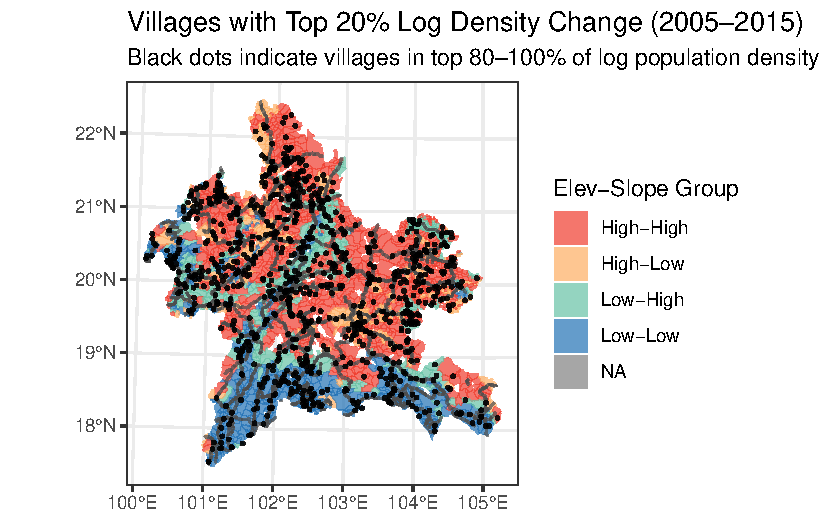
\includegraphics[keepaspectratio]{population_files/figure-pdf/unnamed-chunk-54-1.pdf}}

\pandocbounded{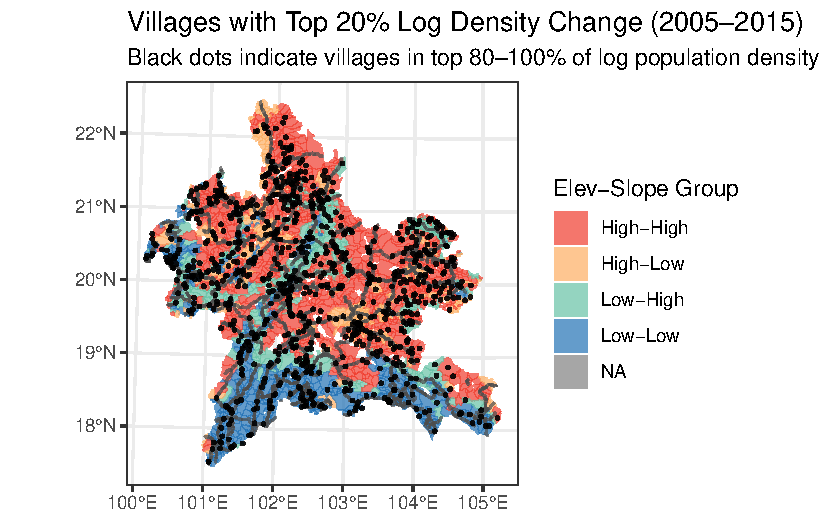
\includegraphics[keepaspectratio]{population_files/figure-pdf/unnamed-chunk-55-1.pdf}}

\begin{longtable}[]{@{}ccccccc@{}}
\caption{Number of Villages by Elevation-Slope Group and Population
Density Change Quantile (log difference, WorldPop)}\tabularnewline
\toprule\noalign{}
elevation\_slope\_group & 0--20\% & 20--40\% & 40--60\% & 60--80\% &
80--100\% & NA \\
\midrule\noalign{}
\endfirsthead
\toprule\noalign{}
elevation\_slope\_group & 0--20\% & 20--40\% & 40--60\% & 60--80\% &
80--100\% & NA \\
\midrule\noalign{}
\endhead
\bottomrule\noalign{}
\endlastfoot
High-High & 327 & 293 & 311 & 335 & 369 & 0 \\
High-Low & 130 & 134 & 158 & 165 & 131 & 0 \\
Low-High & 178 & 175 & 147 & 113 & 105 & 0 \\
Low-Low & 306 & 339 & 326 & 328 & 337 & 0 \\
NA & 1 & 0 & 0 & 0 & 0 & 6 \\
\end{longtable}

\begin{longtable}[]{@{}ccccccc@{}}
\caption{Number of Villages by Elevation-Slope Group and Population
Density Change Quantile (log difference, Matched PHC)}\tabularnewline
\toprule\noalign{}
elevation\_slope\_group & 0--20\% & 20--40\% & 40--60\% & 60--80\% &
80--100\% & NA \\
\midrule\noalign{}
\endfirsthead
\toprule\noalign{}
elevation\_slope\_group & 0--20\% & 20--40\% & 40--60\% & 60--80\% &
80--100\% & NA \\
\midrule\noalign{}
\endhead
\bottomrule\noalign{}
\endlastfoot
High-High & 332 & 295 & 302 & 346 & 360 & 0 \\
High-Low & 135 & 154 & 148 & 147 & 134 & 0 \\
Low-High & 173 & 178 & 143 & 111 & 113 & 0 \\
Low-Low & 301 & 314 & 348 & 337 & 335 & 1 \\
NA & 1 & 0 & 0 & 0 & 0 & 6 \\
\end{longtable}

\phantomsection\label{refs}
\begin{CSLReferences}{1}{0}
\bibitem[\citeproctext]{ref-drug1992opium}
Administration, Drug Enforcement et al. 1992. {``Opium Poppy Cultivation
and Heroin Processing in Southeast Asia.''} \emph{Washington DC: Office
of Intelligence}.

\bibitem[\citeproctext]{ref-cohen2009post}
Cohen, Paul T. 2009. {``The Post-Opium Scenario and Rubber in Northern
Laos: Alternative Western and Chinese Models of Development.''}
\emph{International Journal of Drug Policy} 20 (5): 424--30.

\bibitem[\citeproctext]{ref-lu2019tapping}
Lu, Juliet N. 2019. {``Tapping into Rubber: China's Opium Replacement
Program and Rubber Production in Laos.''} In \emph{De-Centring Land
Grabbing}, 30--51. Routledge.

\bibitem[\citeproctext]{ref-lu2023peripheral}
Lu, Juliet, and Michael B Dwyer. 2023. {``Peripheral Centers: Vertical
Politics and the Geography of Chinese Cross-Border Opium Replacement in
Southeast Asia's {`New Golden Triangle'}.''} \emph{Eurasian Geography
and Economics} 64 (7-8): 811--41.

\bibitem[\citeproctext]{ref-sviatschi2022making}
Sviatschi, Maria Micaela. 2022. {``Making a Narco: Childhood Exposure to
Illegal Labor Markets and Criminal Life Paths.''} \emph{Econometrica} 90
(4): 1835--78.

\bibitem[\citeproctext]{ref-tni2010alternative}
TNI. 2010. {``Alternative Development or Business as Usual.''} In
\emph{Drugs and Democracy}. Transnational Institute.

\bibitem[\citeproctext]{ref-unodc2000opiumsurvey}
UNODC. 2000. {``Laos Opium Survey 2000.''} UNODC.

\bibitem[\citeproctext]{ref-unodc2001opiumsurvey}
---------. 2001. {``Laos Opium Survey 2001.''} UNODC.

\bibitem[\citeproctext]{ref-unodc2005opiumsurvey}
---------. 2005. {``Laos Opium Survey 2005.''} UNODC.

\bibitem[\citeproctext]{ref-unodc2015opiumsurvey}
---------. 2015. {``Southeast Asia Opium Survey 2015.''} UNODC.

\end{CSLReferences}




\end{document}
